\documentclass[11pt, a4paper]{article}

\usepackage{amsmath}
\usepackage[a4paper, margin=1in]{geometry}
\usepackage{amsfonts}
\usepackage{mathtools}
\usepackage{tikz}
\usetikzlibrary{automata, positioning}

\usepackage{pgfplots}
\pgfplotsset{width=5cm,compat=1.9}

% remove paragraph indent
\setlength{\parindent}{0em}

% hyperlinks for the table of contents
% \usepackage{color}
\usepackage{hyperref}
\hypersetup{
    colorlinks=true, % make the links colored
    linkcolor=blue, % color TOC links in blue
    urlcolor=red, % color URLs in red
    linktoc=all % 'all' will create links for everything in the TOC
}

\DeclareMathOperator*{\minimize}{minimize}
\DeclareMathOperator*{\maximize}{maximize}
\DeclareMathOperator*{\argmin}{argmin}
\DeclareMathOperator*{\argmax}{argmax}

\title{Probability Notes}

\begin{document}
    \maketitle{}
    \tableofcontents
    \newpage

    \pagenumbering{arabic}
    \section{Probability Theorems}
    \subsection{Set Theorems}
    For any three sets, the following hold true
    \begin{align*}
        A &= (A \cap B) \cup (A \cap B^{c}) \;where\;B\;and\;B^{c}\;are\;disjoint \\
        A \cap (B \cup C) &= (A \cap B) \cup (A \cap C) \\
        A \cup (B \cap C) &= (A \cup B) \cap (A \cup C)
    \end{align*}

    \subsection{Basic Probability Rules}
    \begin{align*}
        &\text{If } A \cap B = \phi \text{, then } P(A \cup B) = P(A) + P(B)\\
        &P(A|B)P(B) = P(B|A)P(A) = P(A \cap B) \tag*{Bayes' Theorem}\\
        &P(A) = P(A \cap B) + P(A \cap B^{c}) = P(A|B)P(B) + P(A|B^{c})P(B^{c})\\
        &P(A \cap B \cap C) = P(A) P(B|A) P(C|B,A) \tag*{Chain Rule}
    \end{align*}

    \subsubsection{Total Probability Theorem}
    Let $A_{1}$, $A_{2}$, .. ,$A_{n}$ be n disjoint events that completely cover the event space, and B be another event, then
    \begin{align*}
        P(B) &= P(B|A_{1})P(A_{1}) + P(B|A_{2})P(A_{2}) + \cdots + P(B|A_{n})P(A_{n})\\
        \text{or, } P(B) &= \sum_{i=1}^{n} P(B|A_{i})P(A_{i})
    \end{align*}
    \subsection{Independence}
    Two events A and B are independent iff
    \begin{align*}
        &P(A \cap B) = P(A) P(B)
    \end{align*}
    Note that \emph{independence} is not the same as \emph{disjoint}
    \begin{align*}
    A \cap B = \phi \Rightarrow P(A \cap B) = 0 \text{ but } P(A) \neq P(B) \neq 0
    \end{align*}
    Multiple events $A_{1}, A_{2}, \ldots , A_{n}$ are independent iff
    \begin{align*}
        P(A_{i} \cap A_{j} \cap \ldots \cap A_{k}) = P(A_{i}) P(A_{j}) \;..\; P(A_{k}) \;\;\forall\;i,j,\ldots,k \;|\; i,j,\ldots,k \in {1,2,\ldots,n}
    \end{align*}
    Conditional Independence is similar to the above equation. For an event C,
    \begin{align*}
        P(A_{i} \cap A_{j} \cap \ldots \cap A_{k} | C) = P(A_{i}|C) P(A_{j}|C) \;..\; P(A_{k}|C) \;\;\forall\;i,j,\ldots,k \;|\; i,j,\ldots,k \in {1,2,\ldots,n}
    \end{align*}
    
    \subsection{Joint Probability Distributions}
    \emph{Joint Probability Distributions} are defined for two or more than two variables. In this section, we only consider two variables. The formal definition is

    \begin{align*}
        P_{XY}(x, y) = P(X = x \;and\; Y = y)
    \end{align*}

    Based on this definition, the following theorems follow

    \begin{align*}
        \sum_{x} \sum_{y} P_{XY}(x,y) &= 1 \\
        P_{X}(x) &= \sum_{y} P_{XY}(x,y) \tag*{Marginal Probability} \\
        P_{X|Y}(x|y) &= P_{X|Y}(X=x|Y=y) = \frac{P_{XY}(x,y)}{P_{Y}{y}} \\
        \sum_{x} P_{X|Y}(x|y) &= 1 \tag*{Since Y is fixed and we sum over all X's} \\
        P_{XYZ}(x,y,z) &= P_{X}(x) P_{Y|X}(y|x) P_{Z|X,Y}(z|x,y) \tag*{Chain Rule}
    \end{align*}

    \subsection{Expected Value}
    Before going to expected value, let's define a Random Variable
    \begin{align*}
        \text{Random Variable } X \text{ is a linear map : } \mathbb{R} \to \mathbb{R} \text{. The value taken by the variable is denoted by } x
    \end{align*}
    
    $X$ will have an associated probability distribution, i.e., $P_{X}(X = x)$ . Using these quantities, we have
    \begin{align*}
        E[X] = \sum_x xP_{X}(X = x) \tag*{Expected Value}
    \end{align*}

    Based on this definition, the following theorems for expected value follow
    \begin{align*}
        E[\alpha] &= \alpha
        E[\alpha X] &= \alpha E[X] \\
        E[\alpha X + \beta] &= \alpha E[X] + \beta \\
        E[g(X)] &= \sum_x g(x)P_{X}(X = x) \\
        E[X^{2}] &= \sum_x x^{2} P_{X}(X = x) \tag*{Also called \emph{Second Moment}}\\
        E[X|A] &= \sum_{x} x P_{X|A}(X|A) \\
        E[g(X)|A] &= \sum_{x} g(x) P_{X|A}(X|A) \\
        E[X + Y + Z] &= E[X] + E[Y] + E[Z] \tag*{Linearity of Expectation}\\
        E[XY] &= \sum_{X} \sum_{Y} xy P_{XY}(x,y) \\
        E[g(X,Y)] &= \sum_{X} \sum_{Y} g(xy) P_{XY}(x,y) \\
        E[XY] &= E[X]E[Y] \tag*{if X and Y are \emph{independent}}
    \end{align*}
    where $\alpha, \beta \in \mathbb{R}$, $g(X) : \mathbb{R} \rightarrow \mathbb{R}$, and $A$ is an event, $X, Y, Z$ are Random Variables

    \subsubsection{Total Expectation Theorem}
    The \emph{Total Expectation Theorem} is the natural extension of the \emph{Total Probability Theorem}
    Let $A_{1}, A_{2}, \ldots, A_{n}$ be n disjoint events that completely cover the event space, and X be random variable, then
    \begin{align*}
        E[X] &= E[X|A_{1}]P(A_{1}) + E[X|A_{2}]P(A_{2}) + \cdots + E[X|A_{n}]P(A_{n})\\
        \text{or, } E[X)] &= \sum_{i=1}^{n} E[X|A_{i}]P(A_{i})
    \end{align*}

    \subsection{Variance}
    The formal definition of variance is
    \begin{align*}
        Var(X) = E[(X - \bar{X})^{2}] = E[X^{2}] - E[X]^{2}
    \end{align*}
    Using this definition, the following theorems follow
    \begin{align*}
        E[X^{2}] &= E[X]^{2} + Var(X) \\
        Var(\alpha) &= 0 \\
        Var(\alpha X + \beta) &= \alpha^{2} Var(X) \\
        Var(X + Y) &= Var(X) + Var(Y) \text{  if $X$ and $Y$ are \emph{independent} random variables}
    \end{align*}

    \subsection{Cumulative Probability Distribution}
    Cumulative probability distribution is defined for both discrete and continuous variables
    \begin{align*}
        F_{x}(X) = P(X \leq x) = \begin{cases} \int_{-\inf}^{x} p_{X}(t) dt &\mbox{$X$ is a discrete random variable}\\
                                               \sum_{k <= x} P_{X}(k) &\mbox{$X$ is a continuous random variable} \end{cases}
    \end{align*}



    \section{Binomial Random Variable}
    \emph{Binomial Random Variable} $X$ is defined as the number of successes in an experiment with $n$ independent trials, where each trial can only have two outcomes, \emph{success} or \emph{failure}.\\
    Let $X_{i}$ denote the Random Variable corresponding to the individual trials, with probability of success $p$. Then we have the following

    \begin{alignat*}{2}
        X_{i} &= \begin{cases} 1 &\mbox{if success in trial i}\\ 
                                0 &\mbox{otherwise} \end{cases} \tag*{indicator variable} \\
        X &= X_{1} + X_{2} + \cdots + X_{n} = \sum_{i=1}^{n} X_{i} \\
        P(X=k) &= \sum_{k=0}^{n} \binom{n}{k} p^{k} (1 - p)^{n-k}
    \end{alignat*}

    \subsection{Mean and Variance}
    First let's calculate the mean and variance for a single trial $X_{i}$
    \begin{alignat*}{2}
        E[X_{i}] &= 1 * p + 0 * (1 - p) &&= p\\
        Var(X_{i}) &= (1 - p)^{2}p + (0-p)^{2}(1-p) &&= p(1-p)
    \end{alignat*}
    
    We know that all $X_{i}'s$ are independent. Hence, the mean and variance for X become
    \begin{alignat*}{3}
        E[X] &= E[\sum_{i=1}^{n} X_{i}] &&= \sum_{i=1}^{n}E[X_{i}] &&= np \\
        Var(X) &= Var(\sum_{i=1}^{n} X_{i}) &&= \sum_{i=1}^{n} Var(X_{i}) &&= np(1-p)
    \end{alignat*}

    %%%%%%%%%%%%%%%%%%%%%%%%%%%%%%%%%%%%%%%%%%%%%%%%%%%%%%%%%%%%%%%%%%%%%%%%%%%
    \section{Continuous Uniform Random Variable}
    A uniform random variable is defined as follows
    \begin{align*}
        f_{X}(x) = \begin{cases} \frac{1}{b-a} &\mbox{$if a \leq x \leq b$}\\
                                    0 &\mbox{otherwise} \end{cases}
    \end{align*}

    \subsection{Mean and Variance}
    \begin{align*}
        E[X] &= \int_{a}^{b} x \frac{1}{b-a} dx = [\frac{x^{2}}{2(b-a)}]_{a}^{b}\\
            &= \frac{a+b}{2}\\
        Var(X) &= \int_{a}^{b} (x - \frac{a+b}{2})^{2} \frac{1}{b-a} dx \\
            &= \frac{(b-a)^{2}}{12}
    \end{align*}

    %%%%%%%%%%%%%%%%%%%%%%%%%%%%%%%%%%%%%%%%%%%%%%%%%%%%%%%%%%%%%%%%%%%%%%%%%%%
    \section{Gaussian Distribution}
    The gaussian distribution (or normal distribution) is defined between $-\inf$ and $\inf$. It is parametrized by mean $\mu$ and variance $\sigma$, $X \sim \mathcal{N}(\mu, \sigma^{2})$
    \begin{align*}
        f_{X}(x) = \frac{1}{\sqrt{2\pi \sigma^{2}}} e^{-\frac{(x-\mu)^{2}}{2 \sigma^{2}}}
    \end{align*}
    As already described,
    \begin{align*}
        E[X] &= \mu\\
        Var(X) &= \sigma^{2}
    \end{align*}

    A \emph{Standard Normal} is defined as a normal distribution with $\mu = 0$ and $\sigma^{2} = 1$\\
    Any normal distribution can be converted to a standard normal as $X = \frac{X - \mu}{\sigma}$\\
    If $Y = aX + b$, then $Y \sim \mathcal{N}(a \mu + b, a^{2}\sigma^{2})$

    %%%%%%%%%%%%%%%%%%%%%%%%%%%%%%%%%%%%%%%%%%%%%%%%%%%%%%%%%%%%%%%%%%%%%%%%%%%
    \section{Covariance and Correlation}
    For any two random variables X and Y,
    \begin{align*}
        Cov(X,Y) &= E[(X - \overline{X})(Y - \overline{Y})] = E[XY] - E[X]E[Y]\\
        Cov(X,X) &= Var(X)\\
        Corr(X,Y) &= E[(\frac{X - \overline{X}}{\sigma_{X}}) (\frac{Y - \overline{Y}}{\sigma_{Y}})]\\
        &= \frac{Cov(X,Y)}{\sigma_{X} \sigma_{Y}}
    \end{align*}
    Key points to note
    \begin{itemize}
        \item \emph{Inpdependence} $\Rightarrow Cov(X,Y) = Corr(X,Y) = 0$, but the converse is \emph{\textbf{not}} true
        \item Correlation is dimensionless and $-1 \leq Corr(X,Y) \leq 1$ with value close to $0$ implying minimal relation and values close to $-1, 1$ implying perfect relation
    \end{itemize}

    %%%%%%%%%%%%%%%%%%%%%%%%%%%%%%%%%%%%%%%%%%%%%%%%%%%%%%%%%%%%%%%%%%%%%%%%%%%
    \section{Iterated Expectation and Variance}
    The law of iterated expectation tells the following about expectation and variance
    \begin{align*}
        E[E[X|Y]] &= E[X] \\
        Var(X) &= E[Var(X|Y)] + Var(E[X|Y])\\
    \end{align*}

    Proof for Iterated Expectation
    \begin{align*}
        P(X) &= \sum_{y} P(X|Y) P(Y) \\
        \Rightarrow E[X] &= \sum_{x} xP(X) = \sum_{x} \sum{y} xP(X|Y)P(Y) \\
            &= \sum_{y} P(Y) \sum_{x} xP(X|Y) = \sum_{y} P(Y) E[X|Y] \\
        \text{or, } E[X] &= E[E[X|Y]] \tag*{$E[X|Y]$ is a function of $X$ and not $Y$}
    \end{align*}
    
    Proof for Variance
    \begin{align*}
        Var(X) &= E[X^{2}] - E[X]^{2} \\
        Var(X|Y) &= E[(X-\overline{X})^{2}|Y] = E[X^{2}|Y] - E[X|Y]^{2} \tag*{1}\\
        Var[E(X|Y)] &= E[E(X|Y)^{2}] - E[E[X|Y]]^{2}\\
                    &= E[E[(X|Y)]^{2}] - E[X]^{2} \tag*{2}\\
        E[Var(X|Y)] &= E[E[X^{2}|Y]] - E[E[X|Y]^{2}] \tag*{from 1}\\
                    &= E[X^{2}] - E[E[X|Y]^{2}] \tag*{3}\\
        E[Var(X|Y)] + Var(E[X|Y]) &= E[X^{2}] - E[X]^{2} \tag*{adding 2 and 3}\\
                                    &= Var(X)
    \end{align*}

    %%%%%%%%%%%%%%%%%%%%%%%%%%%%%%%%%%%%%%%%%%%%%%%%%%%%%%%%%%%%%%%%%%%%%%%%%%%
    \section{Random number of Random Variables}
    Let $X_{i}$ be independent identically distributed Random Variables and let $Y = \sum_{i=1}^{N} X_{i}$ be the sum of $N$ such random variables where $N$ itself is a random variable. Then,
    \begin{align*}
        Y &= X_{1} + X_{2} + \cdots + X_{N}\\
        E[Y|N=n] &= \sum_{i=1}^{n}E[X_{i}]\\
                &= NE[X]\\
        E[Y] &= E[E[Y|N]] = E[NE[X]]\\
            &= E[N]E[X] \tag*{since $E[X]$ will be a number}\\
        Var(Y) &= E[Var(Y|N)] + Var(E[Y|N])\\
            &= E[NVar(X)] + Var(NE[X])\\
            &= E[N]Var(X) + E[X]^{2}Var(N)
    \end{align*}

    %%%%%%%%%%%%%%%%%%%%%%%%%%%%%%%%%%%%%%%%%%%%%%%%%%%%%%%%%%%%%%%%%%%%%%%%%%%
    \section{Bernoulli Process}
    Bernoulli process falls under the family of random processes, which are random variables continuously evolving over time. Bernoulli process can be described as a sequence of independent Bernoulli trials, where each trial has only two outcomes : success with $P(success) = p$ and failure.
    \begin{alignat*}{2}
        P_{X_{t}}(x_{t}) &= \begin{cases} p &\mbox{if $X_{t} = 1$}\\
                                        1-p &\mbox{if $X_{t} = 0$} \end{cases}\\
        E[X_{t}] &= p\\
        Var(X_{t}) &= p(1-p)
    \end{alignat*}

    \subsection{Mean and Variance}
    Number of successes S in n time slots
    \begin{align*}
        P(S=k) &= \binom{n}{k} p^{k}(1-p)^{n-k}\\
        E[S] &= np\\
        Var(S) &= np(1-p)
    \end{align*}

    \subsection{Interarrival Times (Geometric Random Variable)}
    Let $T_{1}$ denote the number of trials till the first success
    \begin{align*}
        P(T_{1} &= t) &= (1-p)^{t-1}p \tag*{$t \in {1, 2, \ldots}$}\\
        E[T_{1}] &= \frac{1}{p}\\
        Var(T_{1}) &= \frac{1-p}{p^{2}}
    \end{align*}
    This process is memoryless as all future coin flips are independent of whatever has happened till now. Also, the distribution is a \textbf{Geometric Random Variable}.

    \subsection{Sum of Interarrival times}
    We are interested in the total time till k arrivals. Let this random variable be $Y_{k}$
    \begin{align*}
        Y_{k} &= T_{1} + T_{2} + \cdots + T_{k} \tag*{where $T_{i}$'s are i.i.d geometric with parameter $p$}\\
        P(Y_{k} = t) &= P(\text{$k-1$ arrivals between $t=1$ to $t=t$ and last arrival at time $t$})\\
           &= \binom{t-1}{k-1}p^{k}(1-p)^{t-k} \tag*{$\forall\; t \geq k$}\\
        E[Y_{k}] &= \sum_{i=1}{k}E[T_{i}]\\
                &= \frac{k}{p}\\
        Var(Y_{k}) &= \sum_{i=1}^{k}Var(T_{i})\\
                    &= \frac{k(1-p)}{p^{2}}
    \end{align*}


    %%%%%%%%%%%%%%%%%%%%%%%%%%%%%%%%%%%%%%%%%%%%%%%%%%%%%%%%%%%%%%%%%%%%%%%%%%%
    \section{Exponential Distribution}
    Exponential distribution is characterized by the parameter $\lambda$ and has the following probability distribution
    \begin{align*}
        f_{X}(x) = \begin{cases} 0 &\mbox{if $x < 0$}\\
                                \lambda e^{-\lambda x} &\mbox{otherwise} \end{cases}
    \end{align*}

    Exponential distribution is used to represent the interarrival time probability distribution in the context of Poisson Process. The cumulative distribution is given by
    \begin{alignat*}{2}
        F_{X}(x) &= \begin{cases} 0 &\mbox{if $x < 0$}\\
                                1 - e^{-\lambda x} &\mbox{otherwise} \end{cases}\\
        P(X > x) &= \int_{x}^{\inf} \lambda e^{-\lambda x} dx\\
        &= e^{-\lambda x}
    \end{alignat*}

    %%%%%%%%%%%%%%%%%%%%%%%%%%%%%%%%%%%%%%%%%%%%%%%%%%%%%%%%%%%%%%%%%%%%%%%%%%%
    \subsection{Mean and Variance}
    The mean of the distribution is given by
    \begin{align*}
        E[x] &= \int_{0}^{\inf} \lambda x e^{-\lambda x} dx\\
        &= [-x e^{-\lambda x}]_{0}^{\inf} + \int_{0}^{\inf} e^{-\lambda x} dx = \frac{1}{\lambda}\\
        \Aboxed{E[X] &= \frac{1}{\lambda}}
    \end{align*}
    where we used integration by parts, $\int uv' = uv - \int u'v$ and substituted $u = x$ and $v = -e^{-\lambda x}/\lambda$.\newline

    For variance, we first calculate the value of $E[x^{2}]$
    \begin{align*}
        E[x^{2}] &= \int_{0}^{\inf} \lambda x^{2} e^{-\lambda x} dx\\
        &= [-x^{2} e^{-\lambda x}]_{0}^{\inf} + \int_{0}^{\inf} 2x e^{-\lambda x} dx\\
        &= [\frac{-2x e^{-\lambda x}}{\lambda}]_{0}^{\inf} - [\frac{2e^{-\lambda x}}{\lambda^{2}}]_{0}^{\inf}\\
        &= \frac{2}{\lambda^{2}}\\
        Var(X) &= E[X^{2}] - E[X]^{2}\\
        \Aboxed{Var(X) &= \frac{1}{\lambda^{2}}}
    \end{align*}
    The above property can be generalized for the $n$th power as well
    \begin{align*}
        E[X^{n}] = \frac{n!}{\lambda^{n}}
    \end{align*}

    %%%%%%%%%%%%%%%%%%%%%%%%%%%%%%%%%%%%%%%%%%%%%%%%%%%%%%%%%%%%%%%%%%%%%%%%%%%
    \subsection{Memoryless Property}
    A fundamental mathematical property of the exponential distribution is the memoryless property. In summary, this means that whatever has transpired till now will not affect the future distribution. Mathematically $P(T > t+s) is independent of t$
    \begin{align*}
        P(T > t+s | T>t) &= \frac{P(T> t+s \text{ and }T > t)}{P(T > t)}\\
        &= \frac{P(T > t + s)}{P(T > t)}\\
        &= \frac{e^{-\lambda(t+s)}}{e^{-\lambda t}}\\
        &= e^{-\lambda s}\\
        \Aboxed{P(T > t+s | T>t) &= P(T > s)}
    \end{align*}


    %%%%%%%%%%%%%%%%%%%%%%%%%%%%%%%%%%%%%%%%%%%%%%%%%%%%%%%%%%%%%%%%%%%%%%%%%%%
    \section{Poisson Process}
    Poisson process also falls in the realm of random processes but is different from Bernoulli process as it is a continuous time process. This process is very commonly used to model arrival times and number of arrivals in a given time interval.
    \begin{align*}
        P(k, \tau) &= \text{Probability of $k$ arrivals in interval of duration $\tau$}\\
        \sum_{k} P(k, \tau) &= 1 \tag*{for a given $\tau$}
    \end{align*}
    Assumptions
    \begin{itemize}
        \item The Probability is dependent only on $\tau$ and not the \emph{location} of the interval
        \item Number of arrivals in disjoint time intervals are \emph{independent}
    \end{itemize}
    
    \subsection{Derivation from Bernoulli Process}
    For a very small interval $\delta$,
    \begin{alignat*}{2}
        P(k, \delta) &= \begin{cases} 1-\lambda \delta &\mbox{$k = 0$}\\
                                     \lambda \delta &\mbox{$k = 1$}\\
                                     0 &\mbox{$k > 2$} \end{cases} + O(\delta^{2})\\
        \lambda &= \lim_{\delta \to 0}\frac{P(1,\delta)}{\delta} \tag*{arrival rate per unit time}\\
        E[k] &= (\lambda \delta) * 1 + (1-\lambda \delta) * 0\\
            &= \lambda \delta \\
        \tau &= n \delta
    \end{alignat*}
    
    The last equation clearly implies that we can approximate the whole process as a bernoulli process where we have $n$ miniscule time intervals with at most one arrival per interval.
    \begin{align*}
        P(k\; arrivals) &= \binom{n}{k} p^{k} (1-p)^{n-k} \\
            &= \binom{n}{k} (\frac{\lambda \delta}{n})^{k} (1 - \frac{\lambda \delta}{n})^{n-k}\\
        \lambda \tau &= np \tag*{or, arrival rate * time = E[arrivals]}\\
        Poisson &= \lim_{\delta \to 0, n \to \inf} Bernoulli\\
        or,\; P(k, \tau) &= \frac{(\lambda \tau)^{k} e^{-\lambda \tau}}{k!} \tag*{$k = 0,1, \cdots$, for a given $\tau$}\\
        where,\; \sum_{k} P(k, \tau) &= 1 \tag*{for a given $\tau$}
    \end{align*}

    Let $N_{t}$ denote the no of arrivals till time t, then
    \begin{align*}
        E[N_{t}] &= \lambda t\\
        Var(N_{t}) &= \lambda t
    \end{align*}

    \subsection{Time till kth arrival}
    Suppose the $k^{th}$ arrival happens at a time $t$. Then we are saying that there have been $k-1$ arrivals till time $t$ and the $k^{th}$ arrival happens at time $t$ (precisely in an interval of $[t, t+\delta]$). Let $Y_{k}$ be the required time,
    \begin{align*}
        f_{Y_{k}}(t)\delta &= P(t \leq Y_{k} \leq t+\delta)\\
                    &= P(\text{$k-1$ arrivals  in $[0,t]$}) (\lambda \delta)\\
                    &= \frac{(\lambda t)^{k-1}}{(k-1)!}e^{-\lambda t}(\lambda \delta)\\
        f_{Y_{k}}(t) &= \frac{\lambda^{k} t^{k-1}}{(k-1)!}e^{-\lambda t} \tag*{Erland Distribution}
    \end{align*}

    \subsection{Time of 1st Arrival}
    Using the Erlang Distribution described above, we have
    \begin{align*}
        f_{Y_{1}}(t) = \lambda e^{-\lambda t}
    \end{align*}
    $Y_{k} = T_{1} + T_{2} + \cdots + T_{k}$ where all $T_{i}$ are independent and exponential distributions.

    \subsection{Merging of Poisson Processes}
    Merging of two Poisson processes is also a Poisson process. Consider two flasbulbs of Red and Green colours, flashing as Possion processes with rates $\lambda_{1}$ and $\lambda_{2}$. Then the process denoting the combined flashing of the two bulbs is also Poisson.\newline
    Consider a very small interval of time $\delta$. In this small interval, any of the individual bulbs can have at most one flashes (since we ignore higher order terms). Thus, the following four possibilities arise \newline
    \begin{table}[h]
    \centering
    \begin{tabular}{c|c|c}
        0 & $Red$ & $\overline{Red}$\\ \hline
        $Green$ & $\lambda_{1} \delta \lambda_{2} \delta $ & $(1-\lambda_{1}\delta)  \lambda_{2} \delta$\\ \hline
        $\overline{Green}$ & $\lambda_{1} \delta (1-\lambda_{2}\delta) $ & $(1-\lambda_{1}\delta) (1-\lambda_{2}\delta)$ \\
    \end{tabular}
    \caption{Base Probabilities for flashes}
    \end{table}
    \begin{table}[h]
    \centering
    \begin{tabular}{c|c|c}
        0 & $Red$ & $\overline{Red}$\\ \hline
        $Green$ & $0$ & $ \lambda_{2} \delta$\\ \hline
        $\overline{Green}$ & $\lambda_{1} \delta$ & $(1-(\lambda_{1} + \lambda_{2}) \delta)$ \\
    \end{tabular}
    \caption{Probabilities after ignoring $\delta^{2}$ terms}
    \end{table}

    Thus, the combined process is Poisson with parameter $\lambda_{1} + \lambda_{2}$ \newline
    \begin{align*}
    P(\text{arrival happened from first process}) = \frac{\lambda_{1} \delta}{\lambda_{1} \delta + \lambda_2 \delta} = \frac{\lambda_{1}}{\lambda_{1} + \lambda_{2}}
    \end{align*}

    \subsection{Splitting of Poisson Process}
    Suppose we have a Poisson process with parameter $\lambda$ which we split into two processes up and down, with probabilities $p$ and $1-p$. The two resulting processes are also Poisson with different parameters.\newline
    Consider a small time slot of length $\delta$. Then,
    \begin{align*}
        P(\text{arrival in this time slot}) &= \lambda \delta\\
        P(\text{arrival in up slot}) &= \lambda \delta p\\
        P(\text{arrival in down slot}) &= \lambda \delta (1-p)
    \end{align*}
    Thus, up and down are themselves Poisson with parameters $\lambda p$ and $\lambda (1-p)$ respectively.

    \subsection{Random Indcidence for Poisson}
    Suppose we have a Poisson process with parameter $\lambda$ running forever. We show up at a random time instant. What is the length of the chosen interarrival time (the total of the time from the last arrival to the next arrival).\newline
    Let $T_{1}^{'}$ denote the time that has elapsed since the last arrival and $T_{1}$ be the time till the next arrival. Note that the reverse process is also Poisson with the same parameter. Thus,
    \begin{align*}
        E[\text{interarrival time}] = E[T_{1}^{'} + T_{1}] = \frac{1}{\lambda} + \frac{1}{\lambda} = \frac{2}{\lambda}
    \end{align*}

    This may seem paradoxical since the time difference between any two arrivals in a Poisson process is same and it's expected length is $\frac{1}{\lambda}$, whereas we got an interval twice this length. The paradox is resolved by considering the fact that when we choose a random point in time, it is more likely to fall in an interval of larger size than the smaller ones (since probability will be proportional to the length of the interval).\newline

    Consider a separate example where we want to compare two values $E[\text{size of a family}]$ and $E[\text{size of a family of a given person}]$.\newline
    The two value will be different due to the underlying nature of the way experiment is conducted. For the first, we randomly choose families and average their sizes. Here, family of any size is equally likely to be picked. In the second case, we first pick a person from the population, get their family size, and then average the sizes of the families. Note that, this experiment is biased since the we are more likely to select people from larger families (or equivalently, it is more likely that we pick a person from a large family since the probability of picking is proportional to the family size). Hence, the second value will likely be larger and the two quantities are not equal.


    %%%%%%%%%%%%%%%%%%%%%%%%%%%%%%%%%%%%%%%%%%%%%%%%%%%%%%%%%%%%%%%%%%%%%%%%%%%
    \section{Markov Process}
    Markov Process is a discrete time process that is not memoryless. Here the random variable takes several possible states, and the probability distribution is defined in such a way that $P(\text{transition from state 1 to state 2})$ is dependent on state 1.\newline

    Let $X_{n}$ be the random variable denoting the state after n transitions and $X_{0}$ will represent the starting state (which can be given or random). Markov assumption states that \emph{Given the current state, past does not matter}. Armed with these,
    \begin{align*}
        p_{ij} &= P(\text{next state $j$ $|$ current state $i$})\\
        p_{ij} &= P(X_{n+1}=j|X_{n}=i) = P(X_{n+1}=j|X_{n}=i, X_{n-1}, \ldots, X_{0})\\
        r_{ij}(n) &= P(X_{n}=j|X_{0}=i) \tag*{or, in state $j$ after $n$ steps}\\
        r_{ij}(n) &= \sum_{k=1}^{m} r_{ik}(n-1)p_{kj}
    \end{align*}

    \subsection{Recurring and Transient States}
    A state $i$ is called \emph{recurrent} if, starting from $i$, and travelling anywhere, it is always possible to return to $i$. If a state is not recurrent, it is \emph{transient}. States in a recurrent class are periodic if they can be grouped into $d > 1$ groups so that all transitions from one group lead to the next group.

    \subsection{Steady State Probabilities}
    \label{sec_markov_steady}
    Do $r_{ij}(n)$ converge to some $\pi_{j}$ (independent of i) ? \newline
    Yes if,
    \begin{itemize}
        \item recurrent states are all in a single class
        \item single recurrent class is not periodic (otherwise oscillations are possible)
    \end{itemize}
    Assuming yes,
    \begin{align*}
        r_{ij}(n) &= \sum_{k} r_{ik}(n-1)p_{kj}\\
        \lim_{n \to \inf} r_{ij}(n) &= \sum_{k} r_{ik}(n-1)p_{kj}\\
        \pi_{ij} &= \sum_{k} \pi_{ik} p_{kj} \tag*{balance equations} \\
        \sum_{i} \pi_{i} &= 1 \\
        \text{frequency of transitions $k \rightarrow j$} &= \pi_{k} p_{kj} \tag*{in one step}\\
        \text{frequency of transitions into $j$} &= \sum_{k} \pi_{k} p_{kj} \tag*{influx from all connected states}
    \end{align*}

    \subsection{Birth Death Process}
    Consider the checkout counter example. The states are represented by the number of people currently being processed, and we always move $n$ to $[n-1, n, n+1]$, i.e., either the people in the queue decrease by one, remain same or increase by one. Let the probability for moving up be $p$ and moving down be $q$.

    \begin{center}
    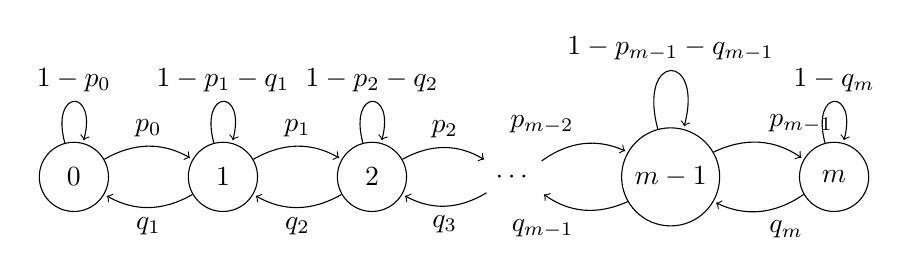
\begin{tikzpicture}
        % first add the node that we want to represent
        \node[state]             (0) {$0$};
        \node[state, right=of 0] (1) {$1$};
        \node[state, right=of 1] (2) {$2$};
        \node[draw=none, right=of 2] (3) {$\cdots$};
        \node[state, right=of 3] (4) {$m-1$};
        \node[state, right=of 4] (5) {$m$};
        % draw the edges between the nodes
        % bend left/right is from the persepective of the starting node
        % and so is the auto=left/right which specifies the side to put text
        \draw[every loop]
            % right edges
            (0) edge[bend left, auto=left] node {$p_{0}$} (1)
            (1) edge[bend left, auto=left] node {$p_{1}$} (2)
            (2) edge[bend left, auto=left] node {$p_{2}$} (3)
            (3) edge[bend left, auto=left] node {$p_{m-2}$} (4)
            (4) edge[bend left, auto=left] node {$p_{m-1}$} (5)
            % left edges
            (1) edge[bend left, auto=left] node {$q_{1}$} (0)
            (2) edge[bend left, auto=left] node {$q_{2}$} (1)
            (3) edge[bend left, auto=left] node {$q_{3}$} (2)
            (4) edge[bend left, auto=left] node {$q_{m-1}$} (3)
            (5) edge[bend left, auto=left] node {$q_{m}$} (4)
            % self loops
            (0) edge[loop above] node {$1-p_{0}$} (0)
            (1) edge[loop above] node {$1-p_{1}-q_{1}$} (1)
            (2) edge[loop above] node {$1-p_{2}-q_{2}$} (2)
            (4) edge[loop above] node {$1-p_{m-1}-q_{m-1}$} (4)
            (5) edge[loop above] node {$1-q_{m}$} (5);
    \end{tikzpicture}
    \end{center}

    Let's estimate the steady state probabilities. Consider the following diagram splitting the chain into two parts through the two adjacent states
    \begin{center}
    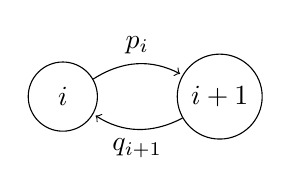
\begin{tikzpicture}
        % first add the node that we want to represent
        \node[state]             (0) {$i$};
        \node[state, right=of 0] (1) {$i+1$};
        % draw the edges between the nodes
        % bend left/right is from the persepective of the starting node
        % and so is the auto=left/right which specifies the side to put text
        \draw[every loop]
            % right edges
            (0) edge[bend left, auto=left] node {$p_{i}$} (1)
            % left edges
            (1) edge[bend left, auto=left] node {$q_{i+1}$} (0);
    \end{tikzpicture}
    \end{center}

    In this case, to maintain steady state, long term frequency of left-right transition should be same as right left transition, i.e., $\pi_{i}p_{i} = \pi_{i+1}q_{i}$ \newline
    In the special case of $p_{i} = p$ and $q_{i} = q \;\forall\; i$,
    \begin{align*}
        \rho &= \frac{p}{q} \tag*{load factor}\\
        \pi_{i+1} &= \pi_{i} \frac{p}{q} = \pi_{i} \rho \\
        \pi_{i} &= \pi_{0} \rho^{i} \tag*{$i = 0,\ldots,m$} \\
        \text{Using } \sum_{i=0}^{m} \pi_{0}\rho^{i} &= 1,\\
        \pi_{0} &= \frac{1}{\sum_{i=0}^{m} \rho^{i}}\\
        \text{if $p < q$ and $m \rightarrow \inf,$}\\
        \pi_{0} &= 1 - \rho \\
        \pi_{i} &= (1-\rho)\rho^{i}\\
        E[X_{n}] &= \frac{\rho}{1-\rho} \tag*{Exponential Distribution}
    \end{align*}
    When $\rho = 1$ or $p = q$, then all states are equally likely - symmetric random walk.

    \subsection{Absorption Probabilities}
    \label{sec_markov_absorb}
    let $a_{i}$ denote the probability of absorption and $\mu_{i}$ denote the expected no of steps until absorption starting from state $i$. Then,
    \begin{align*}
        a_{i} &= \sum_{j} a_{j}p_{ij} \tag*{outflux to the possible states}\\
        \mu_{i} &= 1 + \sum_{j} \mu_{j} p_{ij}
    \end{align*}
    For multipe absorption states, we can possibly consider them together as a group and calculate the relevant quantities. \newline
    For a given state $s$,
    \begin{align*}
        E[\text{steps to first time reach $s$ from $i$}] &= t_{i} \\
        t_{i} &= E[min \{n \geq 0 \text{ such that } X_{n} = s\}] \\
        t_{s} &= 0 \\
        t_{i} &= 1 + \sum_{j} t_{j}p_{ij} \tag*{outflux to all possible states}
    \end{align*}

    Mean recurrence time (mean time to reach back a state) for $s$
    \begin{align*}
        t_{s}^{*} &= E[min\{n \geq 1 \text{ such that } X_{n}=s\} | X_{0} = s] \\
        t_{s}^{*} &= 1 + \sum_{j} t_{j} p_{ij}
    \end{align*}

    %%%%%%%%%%%%%%%%%%%%%%%%%%%%%%%%%%%%%%%%%%%%%%%%%%%%%%%%%%%%%%%%%%%%%%%%%%%
    \section{Central Limit Theorem}
    %%%%%%%%%%%%%%%%%%%%%%%%%%%%%%%%%%%%%%%%%%%%%%%%%%%%%%%%%%%%%%%%%%%%%%%%%%%
    \subsection{Weak Law of Large Numbers}
    Suppose we want to know the mean height of penguins in the world. The absolutely correct answer can be obtained by taking the average of the entire population. But ths is not practical, and often we will have to resort to estimating the quantity through a sample. Let there be $n$ penguins in the sample and $X_{1}, X_{2}, \ldots, X_{n}$ be the random variables denoting their heights. Then,
    \begin{align*}
        M_{n} &= \frac{X_{1} + X_{2} + \cdots + X_{n}}{n}\\
        \lim_{n \to \inf} E[M_{n}] &= E[X] = \text{The true mean}
    \end{align*}

    %%%%%%%%%%%%%%%%%%%%%%%%%%%%%%%%%%%%%%%%%%%%%%%%%%%%%%%%%%%%%%%%%%%%%%%%%%%
    \subsection{Markov Inequality/Chebychev Inequality}
    For nonnegative random variable $X$,
    \begin{alignat*}{2}
        E[X] &= \sum_{x}xp_{X}(x) &&\geq \sum_{x \geq a}xp_{X}(x) \tag*{discrete case}\\
            &= \int_{x}xp_{X}(x) &&\geq \int_{x \geq a}xp_{X}(x) \tag*{continuous case}
    \end{alignat*}
    
    Applying the above set of inequalities to the variable $X - \mu$
    \begin{align*}
        E[(X - \mu)^{2}] &\geq a^{2} P((X - \mu)^{2} \geq a^{2}) \\
        \text{or, \;} Var(X) &\geq a^{2} P(\mid X - \mu \mid \geq a)\\
        \text{For continuous case, }\\
        \sigma^{2} &= \int_{-\inf}^{\inf} (x-\mu)^{2}f_{X}(x) dx\\
                  &\geq \int_{-\inf}^{\mu-c} (x-\mu)^{2}f_{X}(x)dx + \int_{\mu+c}^{\inf} (x-\mu)^{2}f_{X}(x)dx\\
                  &\geq c^{2} P(\mid X - \mu \mid \geq c)\\
        \text{Hence,}\\
        P(\mid X - \mu \mid \geq c^{2}) &\leq \frac{\sigma^{2}}{c^{2}}\\
        \text{or, } \\
        \Aboxed{P(\mid X - \mu \mid \geq k\sigma) &\leq \frac{1}{k^{2}}}\text{\;\;\;where $c = k\sigma$}
    \end{align*}

    Going back to the problem of estimating the mean,
    \begin{align*}
        M_{n} &= \frac{X_{1} + X_{2} + \cdots + X_{n}}{n} \\
        E[M_{n}] &= \frac{1}{n} \sum_{i=1}^{n} E[X_{i}] = \mu \text{\;\; expectation of expectation} \\
        Var(M_{n}) &= \sum_{i=1}^{n} Var(\frac{X_{i}}{n}) = \frac{\sigma^{2}}{n} \text{\;\; since $X_{i}$ are independent} \\
        \Aboxed{P(\mid M_{n} - \mu \mid \geq \epsilon) &\leq \frac{\sigma^{2}}{n\epsilon^{2}}}
    \end{align*}
    or, as $n \rightarrow \inf,\; M_{n} - \mu \rightarrow 0$, $\epsilon$ is the error bound/confidence.

    %%%%%%%%%%%%%%%%%%%%%%%%%%%%%%%%%%%%%%%%%%%%%%%%%%%%%%%%%%%%%%%%%%%%%%%%%%%
    \subsection{Central Limit Theorem}
    Chebychev's inequality gives a loose bound. We can do better with CLT. Let $X$ be a random variable with mean $\mu$ and variance $\sigma^{2}$, and let $X_{i}$ be independent identically distributed random variables with the same distribution as $X$. Then,
    \begin{align*}
        S_{n} &= X_{1} + X_{2} + \cdots + X_{n}\\
        Z_{n} &= \frac{S_{n} - E[S_{n}]}{\sigma_{n}} \text{\;\;random variable with mean $0$ and variance $1$} \\
             &= \frac{S_{n} - nE[X]}{\sqrt{n} \sigma}\\
        \text{or,\;\;} S_{n} &= \sqrt{n} \sigma Z_{n} + nE[X] \\
        \text{In\;\;} \lim_{n \to \inf} Z_{n} &\rightarrow Z \text{\;(standard normal)}\\
        \text{or,\;\;} \Aboxed{Z &= \frac{S_{n} - nE[X]}{\sqrt{n} \sigma}} \text{\;\;only for CDF (no comment on PDF/PMF)}\\
        \text{Thus,\;\;} \Aboxed{P(Z > c) &= P(\frac{S_{n} - nE[X]}{\sqrt{n} \sigma} > c)}
    \end{align*}
    By defining the confidence on how close we desire $S_{n}$ to the actual mean, we can calculate the required value of the $n$ using standard normal CDF tables. However, we need to have an estimate of variance of the distribution in order to do the estimate of $n$.


    %%%%%%%%%%%%%%%%%%%%%%%%%%%%%%%%%%%%%%%%%%%%%%%%%%%%%%%%%%%%%%%%%%%%%%%%%%%
    \section{Bayesian Inference}
    We have a signal $S$ that goes through a "model" $a$ through which we observe $X$ (with sum added noise $N$). The aim of Bayesian Inference is to try to infer $S$ given the observed $X$.
    \newline
    Hypothesis testing is done on an unknown that takes some possible values, and the aim is to arrive at a value that gives a small probability of incorrect decision (e.g. - Radar)
    \newline
    Estimation is aimed at finding the value of a quantity with a small estimation error (e.g. poll estimation)
    \newline
    Bayes Rule
    \begin{align*}
        p_{\Theta|X}(\theta|x) &= \frac{p_{\Theta}(\theta)p_{X|\Theta}(x|\theta)}{p_{X}(x)} \tag*{$\theta$ and $X$ are both discrete}\\
        \text{or,\;\;} Posterior &= \frac{Prior * Model}{Data}\\
        p_{\Theta|X}(\theta|x) &= \frac{p_{\Theta}(\theta)f_{X|\Theta}(x|\theta)}{f_{X}(x)} \tag*{$\theta$ is discrete and $X$ is continuous}\\
    \end{align*}
    Note that Bayesian inference will give us a distribution over the possible values, but it is often desirable to get an estimate.

    \subsection{Maximum a Posteriori (MAP)}
    MAP is a point estimate of the unknown quantity and is defined as follows
    \begin{align*}
        p_{\Theta|X}(\theta|x) = \max_{\theta}p_{\Theta|X}(\theta|x) \tag*{$\theta$ with maximum posterior probability}\\
    \end{align*}
    In continuous case, expected value can be a better estimate

    \subsection{Maximum Likelihood Estimation}
    This is another method to give estimates from the Bayesian Inference. We assume the random variable of interest to be generated through a model with some parameters, i.e. $X \sim p_{X}(x;\theta)$ and we pick the $\theta$ that makes the data most likely
    \begin{align*}
        \hat{\theta}_{MLE} &= \argmax_{\theta} p_{X|\Theta}(x|\theta)\\
        \hat{\theta}_{MAP} &= \argmax_{\theta} p_{\Theta|X}(\theta|x)\\
        &= \argmax_{\theta} p_{X|\Theta}(x|\theta)p_{\Theta}(\theta)
    \end{align*}

    Thus, we can see that if we assume a uniform prior on $\theta$, MAP and MLE estimates are the same. MLE estimates tha maximum through cosideration of multiple probabilistic models. We can get different estimates for different priors.


    \subsection{Least Mean Square Estimate}
    Here, we aim to find an estimate such that
    \begin{align*}
        \theta* &= \min_{c} E[(\Theta - c)^{2}]\\
        E[(\Theta - c)^{2}] &= E[\Theta^{2}] - 2cE[\Theta] + c^{2}\\
        \text{Taking derivative,\;\;} \frac{dE}{dc} &= 0\\
        \Aboxed{c &= E[\Theta]}\\
        \text{In general,\;\;} c &= E[\Theta|X] \tag*{minimizes $E[(\Theta - g(X))^{2}]$ over all estimators $g(X)$ }
    \end{align*}
    $E[\Theta]$ minimizes the least squares estimate
    \newline
    When $X$ is observed, the best estimate simlply becomes $E[\Theta|X]$.


    %%%%%%%%%%%%%%%%%%%%%%%%%%%%%%%%%%%%%%%%%%%%%%%%%%%%%%%%%%%%%%%%%%%%%%%%%%%
    \section{Linear Regression}
    We are given pairs of data $(x_{1},y_{1}), (x_{2},y_{2}), \ldots, (x_{n},y_{n})$ (all independent) where we assume that $x$ and $y$ are governed by the linear relation
    \begin{align*}
        y \approx \theta_{0} + \theta_{1}x
    \end{align*}
    The aim is to determine the model which is parametric consisting of two parameters $\theta_{0}$ and $\theta_{1}$. We find it using the least squares estimate, i.e., minimizing
    \begin{align*}
        \minimize_{\theta_{0}, \theta_{1}} \sum_{i=1}^{n} (y_{i} - \theta_{0} - \theta_{1}x)^{2}
    \end{align*}
    The true model also includes noise and is given by
    \begin{align*}
        Y_{i} = \theta_{0} + \theta_{1}X_{i} + W_{i}
    \end{align*}
    where we assume the noise $W_{i} \sim \mathcal{N}(0, \sigma^{2})$ and is independently and identically distributed. Observing some $X$ and $Y$ is same as observing the noise.
    \begin{align*}
        P(X=x,Y=y) &= P(W=y-\theta_{0}-\theta_{1}x) = \frac{1}{\sqrt{2\pi}} \exp(-\frac{(y-\theta_{0}-\theta_{1}x)^{2}}{2})\\
        P(X_{1}=x_{1},Y_{1}=y_{1}, \ldots, X_{n}=x_{n},Y_{n}=y_{n}) &= \prod_{i=1}^{n} P(X_{1}=x_{i},Y_{i}=y_{i})\\
        &= \prod_{i=1}^{n} W_{i} = \prod_{i=1}^{n} \frac{1}{\sqrt{2\pi}} \exp(-\frac{(y_{i}-\theta_{0}-\theta_{1}x_{i})^{2}}{2})
    \end{align*}
    Maximizing the above product is maximizing the likelihood of the occurrence of the data under the model parameters $\theta_{0}$ and $\theta_{1}$. Since taking log will not change the maxima, we usually maximize the log likelihood
    \begin{align*}
        \maximize_{\theta_{0}, \theta_{1}} \prod_{i=1}^{n} \frac{1}{\sqrt{2\pi}} \exp(-\frac{(y_{i}-\theta_{0}-\theta_{1}x_{i})^{2}}{2}) = \minimize_{\theta_{0}, \theta_{1}} \sum_{i=1}^{n} (y_{i}-\theta_{0}-\theta_{1}x_{i})^{2}
    \end{align*}

    We can take derivatives with respect to the parameters of the above function to get the estimate for the parameters as
    \begin{align*}
        \bar{x} &= \frac{1}{n} \sum_{i=1}^{n} x_{i} \text{, } \bar{y} &= \frac{1}{n} \sum_{i=1}^{n} y_{i}\\
        \hat{\theta}_{1} &= \frac{\sum_{i=1}^{n} (x_{i} - \bar{x}) (y_{i} - \bar{y})}{\sum_{i=1}^{n}(x_{i} - \bar{x})^{2}} = \frac{E[(X-\bar{X})(Y-\bar{Y})]}{E[(X-\bar{X})^{2}]} = \frac{Cov(X,Y)}{Var(X)}\\
        \hat{\theta}_{0} &= \bar{y} - \hat{\theta_{1}} \bar{x}
    \end{align*}

    The above formulae can also be derived if the additives are a function of $X$. Since the linear relationship will still be respected and the loglikelihood can be maximized to get the estimates of the parameters.


    %%%%%%%%%%%%%%%%%%%%%%%%%%%%%%%%%%%%%%%%%%%%%%%%%%%%%%%%%%%%%%%%%%%%%%%%%%%
    \section{Exercises}
    \subsection{Problems}
    \begin{enumerate}
    %%%%%%%%%%%%%%%%%%%%
    \item \hypertarget{q_indcomp}{\textbf{Independence in Complements}}\newline
    Given $A \perp B$, show $A \perp B^{c}$ and $A^{c} \perp B^{c}$. \hyperlink{a_indcomp}{Solution}

    %%%%%%%%%%%%%%%%%%%%
    \item \hypertarget{q_conind}{\textbf{Conditional Independence}}\newline
    $A,B,$ and $C$ are independent with $P(C) > 0$. Show that $A\perp B |C$. \hyperlink{a_conind}{Solution}

    %%%%%%%%%%%%%%%%%%%%
    \item \hypertarget{q_geomeet}{\textbf{Geometry of Meeting}}\newline
    R and J have to meet at a given place and each will arrive at the given place independent of each other with a delay of 0 to 1hr uniformly distributed. The pairs of delays are all equally likely. The first to arrive waits for 15 minutes and leaves. What is the probability of meeting ? \hyperlink{a_geomeet}{Solution}
    
    %%%%%%%%%%%%%%%%%%%%
    \item \hypertarget{q_expfn}{\textbf{Expectation of Function}}\newline
    Let $X$ and $Y$ be random variables with $Y = g(X)$. Show $E[Y] = \sum_{x}g(x)p_{X}(x)$. \hyperlink{a_expfn}{Solution}

    %%%%%%%%%%%%%%%%%%%%
    \item \hypertarget{q_cumuldistfn}{\textbf{Cumulative Distribution Function}}\newline
    A random variable X is a combination of a continuous and discrete distribution as follows
    \begin{align*}
        f_{X}(x) = \begin{cases} 0.5 &\mbox{$a \leq x \leq b$}\\
                                 0.5 &\mbox{x = 0.5}\\
                                 0 &\mbox{otherwise} \end{cases}
    \end{align*}
    Find the Cumulative Distribution of X. \hyperlink{a_cumuldistfn}{Solution}
    
    %%%%%%%%%%%%%%%%%%%%
    \item \hypertarget{q_tossh}{\textbf{Number of tosses till first head}}\newline
    When tossing a fair coin, what is the $E[$\# tosses till the first H$]$. \hyperlink{a_tossh}{Solution}
    
    %%%%%%%%%%%%%%%%%%%%
    \item \hypertarget{q_itrexpproof}{\textbf{Iterated Expectation Proof}}\newline
    For discrete variables, show $E[X] = E[E[X|Y]]$. \hyperlink{a_itrexpproof}{Solution}
    
    %%%%%%%%%%%%%%%%%%%%
    \item \hypertarget{q_itrexpthree}{\textbf{Iterated Expectation for three variables}}\newline
    For three random variables $X$, $Y$ and $Z$, show $E[Z|X] = E[E[Z|X,Y]|X]$. \hyperlink{a_itrexpthree}{Solution}
    
    %%%%%%%%%%%%%%%%%%%%
    \item \hypertarget{q_itrexppractice}{\textbf{Iterated Expectation practice}}\newline
    A class has two sections denoted by the random variable $Y$. Let $X$ denote the quiz score of a student. Given that section 1 has 10 students, section 2 has 20 students, $E[X|Y=1] = 90, E[X|Y=2] = 60, Var(X|Y=1) = 10, Var(X|Y=2) = 20$, find $E[X]$ and $Var(X)$. \hyperlink{a_itrexppractice}{Solution}

    %%%%%%%%%%%%%%%%%%%%
    \item \hypertarget{q_hatproblem}{\textbf{Hat Problem}}\newline
    $n$ people throw their hats in a box and then pick a hat at random. What is the expected number of people who pick their own hat ? \hyperlink{a_hatproblem}{Solution}
    
    %%%%%%%%%%%%%%%%%%%%
    \item \hypertarget{q_breakstick}{\textbf{Breaking a stick}}\newline
    A stick of length $l$ is broken first at $X$ uniformly chosen between $[0,l]$, and then at $Y$, uniformly chosen between $[0,X]$. Find the expected length of the shorter part. \hyperlink{a_breakstick}{Solution}

    
    %%%%%%%%%%%%%%%%%%%%
    \item \hypertarget{q_trianglestick}{\textbf{Triangles from a Stick}}\newline
    We have a stick of length 1. We randomly choose two points on the stick and break the stick at those points. Calculate the probability that the three pieces form a triangle. \hyperlink{a_trianglestick}{Solution}


    %%%%%%%%%%%%%%%%%%%%
    \item \hypertarget{q_pmffn}{\textbf{PMF of g(X)}}\newline
    Let $X$ be uniform in $[0, 2]$, then find the PMF of $Y = X^{3}$. \hyperlink{a_pmffn}{Solution}

    %%%%%%%%%%%%%%%%%%%%
    \item \hypertarget{q_waittaxi}{\textbf{Waiting for Taxi}}\newline
    A taxi stand and bus stop near Al's home are at the same location. Al goes there and if a taxi is waiting $P=\frac{2}{3}$, he boards it. Otherwise, he waits for a taxi or bus to come, whichever is first. Taxi takes anywhere between $0$ to $10$ mins (uniform) while a bus arrives in exactly 5 mins. He boards whichever is first. Find CDF and $E$[wait time]. \hyperlink{a_waittaxi}{Solution}
    
    %%%%%%%%%%%%%%%%%%%%
    \item \hypertarget{q_bayes}{\textbf{Bayes Theorem}}\newline
    Let $Q$ be a continuous random variable with PDF
    \begin{align*}
        f_{Q}(q) = \begin{cases} 6q(1-q) &\mbox{ $0 \leq q \leq 1$}\\
                                 0 &\mbox{ otherwise} \end{cases}
    \end{align*}
    where $Q$ represents $P(success)$ for a Bernoulli $X$, i.e., $P(X=1|Q=q) = q$. Find $f_{Q|X}(q|x) \forall x \in [0,1] and q$. \hyperlink{a_bayes}{Solution}
    
    %%%%%%%%%%%%%%%%%%%%
    \item \hypertarget{q_normaltr}{\textbf{A Normal Transformation}}\newline
    Let $X \sim \mathcal{N}(0,1)$ and $Y = g(X)$. Find $p_{Y}(y)$. 
    \begin{align*}
        g(t) = \begin{cases} -t &\mbox{$t \leq 0$}\\
                            \sqrt{t} &\mbox{$t > 0$} \end{cases}
    \end{align*}
    \hyperlink{a_normaltr}{Solution}

    %%%%%%%%%%%%%%%%%%%%
    \item \hypertarget{q_binshoot}{\textbf{Binomial Shooter}}\newline
    A shooter takes 10 hits in a shooting range and each shot has $p=0.2$ of hitting target independent of each other. Let $X = $ number of hits. Find
    \begin{enumerate}
         \item PMF of $X$
         \item $P(no\;hits)$
         \item $P(scoring\;more\;than\;misses)$
         \item $E[X]$ and $Var(X)$
         \item Suppose the entry is \$3 and each shot fetches \$2. Let $Y$ = profit. Find $E[Y] and Var(Y)$.
         \item Suppose entry is free and total reward is square of number of hits. Let $Z$ be profit. Find $E[Z]$.
    \end{enumerate} \hyperlink{a_binshoot}{Solution}

    %%%%%%%%%%%%%%%%%%%%
    \item \hypertarget{q_mosquito}{\textbf{Mosquito and Tick}}\newline
    Every second, a mosquito lands with $P = 0.5$. Once it lands, it bites with $P=0.2$. Let $X$ be the time between successive mosquito bites. Find $E[X]$ and $Var(X)$.\newline
    Now suppose a tick comes into play independent of mosquito. It lands with $P=0.1$ and once landed, bites with $)=0.7$. Let $Y$ be the time between successive bug bites. Find $E[Y]$ and $Var(Y)$. \hyperlink{a_mosquito}{Solution}

    %%%%%%%%%%%%%%%%%%%%
    \item \hypertarget{q_hhtt}{\textbf{HH or TT}}\newline
    Given a coin with $P(H) = p$, find the $E$[number of tosses till $HH$ or $TT$]. \hyperlink{a_hhtt}{Solution}

    %%%%%%%%%%%%%%%%%%%%
    \item \label{itm:threecoins} \hypertarget{q_threecoins}{\textbf{A Three Coin Game}}\newline
    Let $3$ fair coins be tossed at every turn. Given all coins and turns are independent, calculate the following (assuming success is defined as all three coins landing the same side up))
    \begin{enumerate}
        \item PMF of $K$, no of trials upto but not including the $2^{nd}$ success
        \item $E$ and $Var$ of $M$, the $E[$number of tails$]$ before first success.
    \end{enumerate}
    \hyperlink{a_threecoins}{Solution}


    %%%%%%%%%%%%%%%%%%%%
    \item \hypertarget{q_linexp}{\textbf{Linear Expectations}}\newline
    Bob conducts trials in a similar manner to Problem \ref{itm:threecoins}, but with four coins. He repeatedly removes a coin at success until just a single coin remains. Calculate the Expected number of tosses till the finish of experiment. \hyperlink{a_linexp}{Solution}
    

    %%%%%%%%%%%%%%%%%%%%
    \item \hypertarget{q_papers}{\textbf{Papers Drawn with Replacement}}\newline
    Suppose there are $n$ papers in a drawer. We take one paper, sign it, and then put it back into the drawer. We take one more paper out and if it is not signed, we sign it and put it back in the drawer. If the paper is already signed, we simply put it back in the drawer. We repeat this process until all the papers are signed. Find the $E[$papers drawn till all papers are signed$]$. What is the value of this quantity as $n \to large$. \hyperlink{a_papers}{Solution}

    
    %%%%%%%%%%%%%%%%%%%%
    \item \hypertarget{q_threevar}{\textbf{A Three Variable Inequality}} \newline
    Let $X$, $Y$, $Z$ be three exponentially distributed random variables with parameters $\lambda, \mu,$ and $\nu$ respectively. Find $P(X < Y < Z)$. \hyperlink{a_threevar}{Solution}


    %%%%%%%%%%%%%%%%%%%%
    \item \hypertarget{q_poissonemails}{\textbf{Poisson Emails}}\newline
    You get emails according to a Poisson process at the rate of 5 messages/hour. You check email every 30 minutes. Find
    \begin{itemize}
        \item P(no new message)
        \item P(one new message)
    \end{itemize}
    \hyperlink{a_poissonemails}{Solution}

    %%%%%%%%%%%%%%%%%%%%
    \item \hypertarget{q_poissonfish}{\textbf{Poisson Fishing}}\newline
    We go fishing where we catch fishes at the rate of $0.6/hour$. We fish for two hours. If we do not catch a fish in the first two hours, we fist until the first catch. Find the following
    \begin{itemize}
        \item P(fish for $> 2$ hours)
        \item P(fish for $> 2$ but $< 5$ hours)
        \item P(catch at least two fish)
        \item E[fish]
        \item E[Total fishing time]
        \item E[future fishing time|fished for two hours]
    \end{itemize}
    \hyperlink{a_poissonfish}{Solution}

    %%%%%%%%%%%%%%%%%%%%
    \item \hypertarget{q_poissonbulb}{\textbf{Poisson Lightbulbs}}\newline
    We have three identical but independent lightbulbs whose lifetimes are modelled by a Poisson process with parameter $\lambda$. Given that we start all the three bulbs together, find the $E[\text{time until last bulb dies out}]$. \hyperlink{a_poissonbulb}{Solution}


    %%%%%%%%%%%%%%%%%%%%
    \item \hypertarget{q_poissonbulb2}{\textbf{Two Poisson Lightbulbs}}\newline
    Beginning at $t=0$, we begin using bulbs one at a time until failure. Any broken bulb is immediately replaced. Each new bulb is selected independently and equally likely from type A(exponential life with $\lambda = 1$) or type B(exponential life with $\lambda = 3$). Lifetimes of all bulbs are independent.
    \begin{enumerate}
        \item Find $E[$time until first failure$]$.
        \item $P($no bulb failure before time $t)$.
        \item Given that there are no failures until time t, determine the conditional probability that the first bulb used is of type A.
        \item Find the probability that the total illumination by two type B bulbs $>$ one type A.
        \item Suppose the process terminates after 12 bulbs fail. Determine the expected value and variance of the total illumination provided by type B bulbs while the process is in operation.
        \item Given there are no failures until time $t$, find the expected value of time until first failure.
    \end{enumerate}
    \hyperlink{a_poissonbulb2}{Solution}

    %%%%%%%%%%%%%%%%%%%%
    \item \hypertarget{q_steadymarkov}{\textbf{Steady State Markov Process}}\newline
    Find the steady state probabilites of the following Markov Process\newline
    \begin{center}
    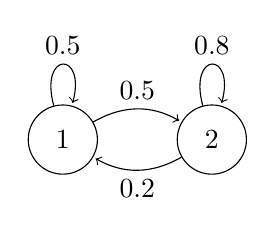
\begin{tikzpicture}
        % first add the node that we want to represent
        \node[state]             (1) {$1$};
        \node[state, right=of 1] (2) {$2$};
        % draw the edges between the nodes
        % bend left/right is from the persepective of the starting node
        % and so is the auto=left/right which specifies the side to put text
        \draw[every loop]
            % right edges
            (1) edge[bend left, auto=left] node {$0.5$} (2)
            % left edges
            (2) edge[bend left, auto=left] node {$0.2$} (1)
            % self loops
            (1) edge[loop above] node {$0.5$} (1)
            (2) edge[loop above] node {$0.8$} (2);
    \end{tikzpicture}
    \end{center}
    \hyperlink{a_steadymarkov}{Solution}

    %%%%%%%%%%%%%%%%%%%%
    \item \hypertarget{q_absorbmarkov}{\textbf{Absorption Probabilities}}\newline
    \begin{center}
    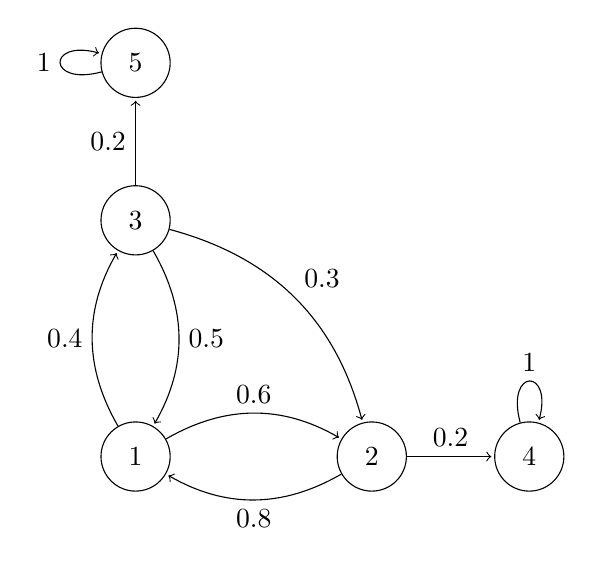
\begin{tikzpicture}
        % first add the node that we want to represent
        \node[state] at (0,0)     (5) {$5$};
        \node[state] at (0,-2)    (3) {$3$};
        \node[state] at (0,-5)    (1) {$1$};
        \node[state] at (3,-5)    (2) {$2$};
        \node[state] at (5,-5)    (4) {$4$};
        % draw the edges between the nodes
        % bend left/right is from the persepective of the starting node
        % and so is the auto=left/right which specifies the side to put text
        \draw[every loop]
            % 5
            (5) edge[loop left] node {$1$} (5)
            % 3
            (3) edge[auto=left]            node {$0.2$} (5)
            (3) edge[bend left, auto=left] node {$0.5$} (1)
            (3) edge[bend left, auto=left] node {$0.3$} (2)
            % 1
            (1) edge[bend left, auto=left] node {$0.4$} (3)
            (1) edge[bend left, auto=left] node {$0.6$} (2)
            % 2
            (2) edge[bend left, auto=left] node {$0.8$} (1)
            (2) edge[auto=left]            node {$0.2$} (4)
            %4
            (4) edge[loop above] node {$1$} (4);
    \end{tikzpicture}
    \end{center}    
    Calculate the absorption probabilites for state $4$ and expected time to absortion from all states. (for absorption time, assume $p_{35} = 0$ and $p_{32} = 0.5$) \hyperlink{a_absorbmarkov}{Solution}

    %%%%%%%%%%%%%%%%%%%%
    \item \hypertarget{q_markovcourse}{\textbf{Selecting Courses with Markov Process}}\newline
    \begin{center}
    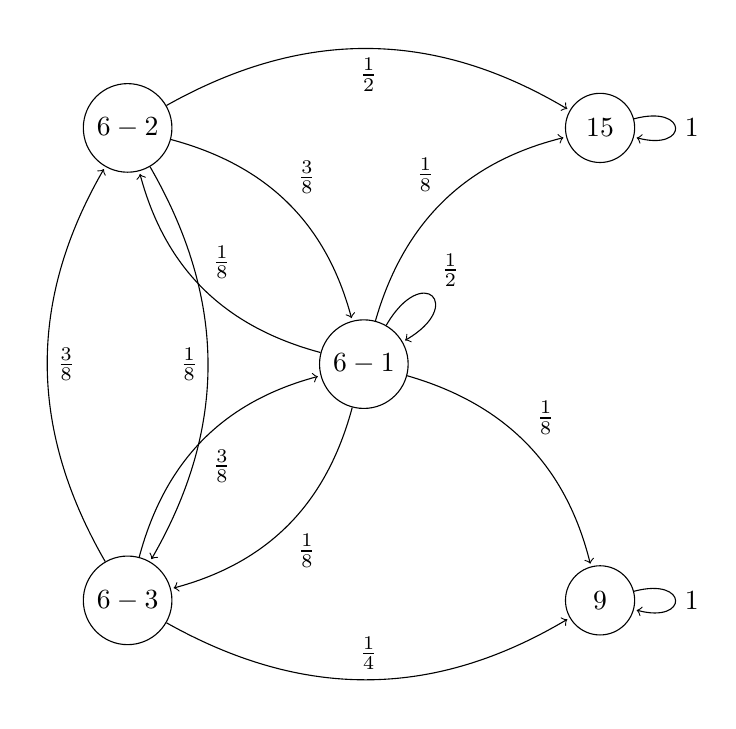
\begin{tikzpicture}
        % first add the node that we want to represent
        \node[state] at (0,0)     (61) {$6-1$};
        \node[state] at (-3,3)    (62) {$6-2$};
        \node[state] at (3,3)     (15) {$15$};
        \node[state] at (-3,-3)   (63) {$6-3$};
        \node[state] at (3,-3)    (9) {$9$};
        % draw the edges between the nodes
        % bend left/right is from the persepective of the starting node
        % and so is the auto=left/right which specifies the side to put text
        \draw[every loop]
            % 6-1
            (61) edge[out=60, in=30, loop, auto=left] node {$\frac{1}{2}$} (61)
            (61) edge[bend left, auto=right] node {$\frac{1}{8}$} (62)
            (61) edge[bend left, auto=left] node {$\frac{1}{8}$} (63)
            (61) edge[bend left, auto=left] node {$\frac{1}{8}$} (9)
            (61) edge[bend left, auto=left] node {$\frac{1}{8}$} (15)
            % 6-2
            (62) edge[bend left, auto=left] node {$\frac{3}{8}$} (61)
            (62) edge[bend left, auto=right] node {$\frac{1}{8}$} (63)
            (62) edge[bend left, auto=right] node {$\frac{1}{2}$} (15)
            %6-3
            (63) edge[bend left, auto=right] node {$\frac{3}{8}$} (61)
            (63) edge[bend left, auto=right] node {$\frac{3}{8}$} (62)
            (63) edge[bend right, auto=left] node {$\frac{1}{4}$} (9)
            % 9
            (9) edge[loop right] node {$1$} (9)
            % 15
            (15) edge[loop right] node {$1$} (15);
    \end{tikzpicture}
    \end{center}

    Consider the above markov process for changing courses. The probability being in some course tomorrow given a course today is mentioned along the edges. Suppose we start with course 6-1 (Note that course 6 is the combination of courses 6-1, 6-2 and 6-3). Calculate the following
    \begin{enumerate}
        \item $P($eventually leaving course 6$)$.
        \item $P($eventually landing in course 15$)$.
        \item $E[$number of days till leaving course 6$]$.
        \item At every switch for 6-2 to 6-1 or 6-3 to 6-1, we buy an ice cream (but a maximum of two). Calculate the $E[$number of ice creams before leaving course 6$]$.
        \item Suppose we end up in 15. What is the $E[$number of steps to reach 15$]$.
        \item Suppose we don't want to take course 15. Accordingly, when in 6-1, we stay there with probability $1/2$ while other three options have equal probabilities. If we are in 6-2, probability of going to 6-1 and 6-3 are in the same ratio as before. Calculate the $E[$number of days until we enter course 9$]$.
        \item Assuming $P(X_{n+1}=15|X_{n}=9) = P(X_{n+1}=9|X_{n}=15) = P(X_{n+1}=15|X_{n}=15) = P(X_{n+1}=9|X_{n}=9) = 1/2$, what is $P(X_{n}=15)$ and $P(X_{n}=9)$ far into the future.
        \item Suppose $P(X_{n+1}=6-1|X_{n}=9) = 1/8, P(X_{n+1}=9|X_{n}=9) = P(X_{n+1}=15|X_{n}=15) = 7/8$. What is the $E[$number of days till return to 6-1$]$.
    \end{enumerate}  

    \hyperlink{a_markovcourse}{Solution}


    %%%%%%%%%%%%%%%%%%%%
    \item \hypertarget{q_binclt}{\textbf{Estimating Binomial with CLT, 1/2 correction}}\newline
    Given a Bernoulli Process with $n = 36$ and $p = 0.5$, find $P(S_{n} \leq 21)$. \hyperlink{a_binclt}{Solution}

    
    %%%%%%%%%%%%%%%%%%%%
    \item \hypertarget{q_mleestimate}{\textbf{MLE Estimate}}\newline
    Suppose we observe $n$ independent and identically distributed samples $x_{1}, x_{2}, \ldots, x_{n}$ from an exponential distribution. Estimate the parameter of the exponential.
    

    %%%%%%%%%%%%%%%%%%%%
    \item \hypertarget{q_lmsestimate}{\textbf{LMS Estimate}}\newline
    Given the prior $f_{\Theta|(\theta)}$, uniform in $[4,10]$, and $f_{X|\Theta}(x|\theta)$ is uniform in $[\theta-1, \theta+1]$, estimate the posterior of $\theta$. \hyperlink{a_lmsestimate}{Solution}

    \item \hypertarget{q_convergence}{\textbf{Probability Convergence}}\newline
    Let $X$ be uniformly distributed between $[-1,1]$. Let $X_{1}, X_{2},\ldots,X_{n}$ be independently and identically distributed with the same distribution as $X$. Find whether the following sequences are convergent in probability and also find the limit.
    \begin{enumerate}
        \item $X_{i}$
        \item $Y_{i} = X_{i}/i$
        \item $Z_{i} = (X_{i})^{i}$
    \end{enumerate}

    %%%%%%%%%%%%%%%%%%%%
    \end{enumerate}


    \subsection{Solutions}
    \begin{enumerate}
        %%%%%%%%%%%%%%%%%%%%
        \item \hypertarget{a_indcomp}{\hyperlink{q_indcomp}{Question}}
        \begin{enumerate}
            \item 
            \begin{align*}
                P(A \cap B) &= P(A) P(B)\\
                P(A) &= P((A \cap B) \cup (A \cap B^{c}))\\
                    &= P(A \cap B) + P(A \cap B^{c}) \tag*{since disjoint}\\
                P(A \cap B^{c}) &= P(A) - P(A)P(B)\\
                    &= P(A)(1 - P(B)) = P(A)P(B^{c})
            \end{align*}
            \item 
            \begin{align*}
                (A \cup B)^{c} &= A^{c} \cap B^{c}\\
                P(A^{c} \cap B^{c}) &= 1 - P(A \cup B)\\
                                &= 1 - P(A) - P(B) + P(A \cap B)\\
                                &= (1 - P(A))(1 - P(B))\\
                                &= P(A^{c})P(B^{c})
            \end{align*}
        \end{enumerate}

        %%%%%%%%%%%%%%%%%%%%
        \item \hypertarget{a_conind}{\hyperlink{q_conind}{Question}}
        \begin{align*}
            P(A \cap B | C) = \frac{P(A \cap B \cap C)}{P(C)} = P(A)P(B) = P(A|C)P(B|C) \tag*{Due to independence}
        \end{align*}

        %%%%%%%%%%%%%%%%%%%%
        \hypertarget{a_geomeet}{\item} \hyperlink{q_geomeet}{Question} \newline
        Suppose R arrives at $x$ hours. J has to arrive between $x$ hrs to $x$ hrs + 15 mins. Similarly if J arrives at $y$ hours, R has to arrive between $y$ hours to $y$ hours + 15 mins. These are regions enclosed by the regions $x \leq 1, y \leq 1, y \leq x + \frac{1}{4} \;and\; y \geq x - \frac{1}{4}$. The probability is then $ 1 - P(not\;meeting) = 1 - 2(\frac{1}{2} \frac{3}{4} \frac{3}{4}) = \frac{7}{16}$.
    
        %%%%%%%%%%%%%%%%%%%%
        \hypertarget{a_expfn}{\item} \hyperlink{q_expfn}{Question}
        \begin{align*}
            E[Y] = \sum_{y}yp_Y(y) = \sum_{y}\sum_{x:g(x)=y}p_{X}(x) = \sum_{y} \sum_{x:g(x)=y} yp_{X}(x)\\
            = \sum_{y} \sum_{x:g(x)=y}g(x)p_{X}(x) = \sum_{x}g(x)p_{X}(x) 
        \end{align*}
    
        %%%%%%%%%%%%%%%%%%%%
        \hypertarget{a_cumuldistfn}{\item} \hyperlink{q_cumuldistfn}{Question} \newline
        Cumulative Distribution of X can be found by integration and is as follows
        \begin{align*}
            f_{X}(x) = \begin{cases} 0 &\mbox{$x < 0$}\\
                                     0.5x &\mbox{$0 \leq x < 0.5$}\\
                                     0.75 &\mbox{x = 0.5}\\
                                     0.75 + 0.5(x-0.5) &\mbox{$0.5 < x \leq 1$} \\
                                     1 &\mbox {$1 < x$}\end{cases}
        \end{align*}
        
        %%%%%%%%%%%%%%%%%%%%
        \hypertarget{a_tossh}{\item} \hyperlink{q_tossh}{Question} \newline
        Let $X$ be the \# of tosses till first \emph{H}. Then, $(X = 1) \cap (X > 1) = \phi$.
        Using \emph{Total Expectation Theorem}
        \begin{align*}
            E[X] &= P(X = 1)E[X|X = 1] + P(X > 1)E[X|X > 1] \\
            &= 0.5 * 1 + 0.5 E[X] \\
            \Rightarrow E[X] &= 2
        \end{align*}
        $P(X = 1) = 0.5$ because then we get the head in the first toss itself. Since $P(X = 1) + P(X > 1) = 1$, we have $P(X > 1) = 0.5$. $E[X] = E[X|X > 1]$ because the tosses are \emph{independent} and thus memoryless.

        %%%%%%%%%%%%%%%%%%%%
        \hypertarget{a_itrexpproof}{\item} \hyperlink{q_itrexpproof}{Question} \newline
        Note that $E[X|Y]$ is a function of $y$.
        \begin{align*}
            E[E[X|Y]] &= \sum_{y} E[X|Y] p_Y(y)\\
                     &= \sum_{y} \sum_{x} xp_{X|Y}p_{Y}\\
                     &= \sum_{y}\sum_{x} xp_{X,Y}(x,y)\\
                     &= \sum_{x}x\sum_{y}p_{X,Y}(x,y)\\
                     &= \sum_{x} x p_{X}(x)\\
                     &= E[X]
        \end{align*}


        %%%%%%%%%%%%%%%%%%%%
        \hypertarget{a_itrexpthree}{\item} \hyperlink{q_itrexpthree}{Question} \newline
        Note that $E[Z|X,Y]$ will be a function of both $X$ and $Y$.
        \begin{align*}
            E[Z|X,Y] &= \sum_{z} z p_{Z|X,Y}(z|x,y)\\
            E[E[Z|X,Y]|X] &= \sum_{y} E[Z|X,Y]p_{X,Y|X}(x,y|x)\\
                        &= \sum_{y} \sum_{z} z p_{Z|X,Y}(z|x,y) p_{Y|X}(y|x)\\
                        &= \sum_{y} \sum_{z} z \frac{p_{X,Y,Z}(x,y,z)}{p_{X}(x)}\\
                        &= \sum_{z} z \sum_{y} \frac{p_{X,Y,Z}(x,y,z)}{p_{X}(x)}\\
                        &= \sum_{z} z \frac{p_{X,Z}(x,z)}{p_{X}(x)}\\
                        &= \sum_{z} z p_{Z|X}(z|x)\\
                        &= E[Z|X]
        \end{align*}

    
        %%%%%%%%%%%%%%%%%%%%
        \hypertarget{a_itrexppractice}{\item} \hyperlink{q_itrexppractice}{Question}\newline
        We use the formulae from iterated expectation to calculate these.
        \begin{alignat*}{2}
            P_{Y}(y) &= \begin{cases} \frac{1}{3} &y = 1\\
                                    \frac{2}{3} &y = 2 \end{cases}\\
            E[X] &= E[E[X|Y]] = \sum_{y}E[X|Y]P(Y)\\
                &= 90 * \frac{1}{3} + 60 * \frac{2}{3}\\
            Var(X) &= E[Var(X|Y)] + Var(E[X|Y])\\
                  &= \sum_{y}Var(X|Y)P(Y) + ((90-E[E[X|Y])^{2}\frac{1}{3} + (60-E[E[X|Y]])^{2}\frac{2}{3})\\
                  &= \frac{650}{3}
        \end{alignat*}
        
        %%%%%%%%%%%%%%%%%%%%
        \hypertarget{a_hatproblem}{\item} \hyperlink{q_hatproblem}{Question}\newline
        Let $X$ denote the number of people who pick their own hat. We have been asked $E[X]$.\\
        Let $X_{i}$ be a binary random variable denoting whether the $i^{th}$ person picked their own hat, i.e.,
        \begin{alignat*}{2}
            X_{i} &= \begin{cases} 1 &\mbox{if $i^{th}$ person picks their own hat}\\ 
                                    0 &\mbox{otherwise} \end{cases} \\
            P(X_{i} = 1) &= \frac{1}{n} \\
            E[X_{i}] &= 1 * \frac{1}{n} + 0 * (1 - \frac{1}{n}) = \frac{1}{n}\\
        \end{alignat*}
        Consequently
        \begin{align*}
            E[X] = E[\sum_{i=1}^{n} X_{i}] = \sum_{n=1}^{n}E[X_{i}] = 1
        \end{align*}

        It is interesting to see the variance of X. Note that the formula for variance is $E[X^{2}] - E[X]^{2}$. Thus,
        \begin{align*}
            X^{2} = (\sum_{i=1}^{n} X_{i})^{2} = \sum_{i=1}^{n} X_{i}^{2} + \sum_{i=1}^{n} \sum_{j=1, j\neq i}^{n} X_{i}X{_j} \\
            E[X^{2}] = \sum_{i=1}^{n}E[X_{i}^{2}] + \sum_{i=1}^{n} \sum_{j=1, j\neq i}^{n} E[X_{i}X{_j}] 
        \end{align*}
        Note that $X_{i}$ and $X_{j}$ are not independent since after the first person has picked the hat, only $n-1$ hats remain
        \begin{alignat*}{3}
            X_{i}X_{j} &= \begin{cases} 1 &\mbox{if $X_{i} = X_{j} = 1$}\\
                                       0 &\mbox{otherwise} \end{cases} \\
            P(X_{i}X_{j} = 1) &= P(X_{i} = 1) P(X_{j} = 1|X_{i} = 1) &&= \frac{1}{n} * \frac{1}{n-1}\\
            E[X_{i}X_{j}] &= 1 * (\frac{1}{n} * \frac{1}{n-1}) + 0 * (1 - \frac{1}{n} * \frac{1}{n-1}) &&= \frac{1}{n(n-1)}\\
            E[X_{i}^2] &= 1^{2} \frac{1}{n} + 0^{2} (1-\frac{1}{n}) &&= \frac{1}{n}
        \end{alignat*}
        Putting these values in the original equation for variance
        \begin{alignat*}{2}
            E[X_{2}] &= n \frac{1}{n} + \frac{1}{n} \frac{1}{n-1} (\frac{n(n-1)}{2} * 2) &&= 2\\
            Var(X) &= 2 - 1^{2} &&= 1
        \end{alignat*}
        

        %%%%%%%%%%%%%%%%%%%%
        \hypertarget{a_breakstick}{\item} \hyperlink{q_breakstick}{Question}\newline
        The following is the joint probability distribution of $X$ and $Y$
        \begin{align*}
            f_{XY}(x, y) = f_{X}(x) f_{Y|X}(y|x) = \frac{1}{l} \frac{1}{x} = \frac{1}{xl} \;\forall\; 0 \leq y \leq x \leq 1
        \end{align*}
        
        Using marginal probabilities, we can calculate $f_{Y}(y) and E[Y] as$
        \begin{align*}
            f_{Y}(y) = \int f_{XY}(x,y) dx = \int_{y}^{l} \frac{1}{xl} dx = \frac{1}{l} \log \frac{l}{y} \tag*{Note that for any $y$, $y \leq x \leq l$}\\
            E[Y] = \int y f_{Y}(y) = \int_{0}{l} y \frac{1}{l} \log\frac{l}{y} = \frac{l}{4}
        \end{align*}

        This problem can also be approched using iterated expectation
        \begin{align*}
            E[Y] &= E[E[Y|X]] = E[\text{uniform random variable between $0$ and $x$}]\\
                &= E[\frac{X}{2}] =\frac{1}{2}E[X]\\
                &= \frac{l}{4} 
        \end{align*}

        %%%%%%%%%%%%%%%%%%%%
        \hypertarget{a_trianglestick}{\item} \hyperlink{q_trianglestick}{Question}\newline
        Assume that we break the stick at points $X$ and $Y$. Assume $X < Y$. Then for the stick to form a triangle, the three lengths $X, Y-X$ and $1-Y$ should satisfy the following three inequalities
        \begin{align*}
            X+(Y-X) &> 1-Y\\
            (Y-X) + (1-Y) &> X\\
            X + (1-Y) &> Y-X
        \end{align*}
        which is nothing but the triangluar region between the points $(0, 0.5), (0.5, 0.5)$ and $(0.5, 1)$ and has the area of $1/8$. We should also consider the case $Y < X$ and by symmetry, the area is same. Now, $X$ and $Y$ comprise of the entire square region $X \leq 1$ and $Y \leq 1$. Hence the required probability is $2 * 1/8 = 1/4$.

        %%%%%%%%%%%%%%%%%%%%
        \hypertarget{a_pmffn}{\item} \hyperlink{q_pmffn}{Question}\newline
        Always solve such questions using the cumulative distribution approach.
        \begin{alignat*}{2}
            P(X \leq x) &= \begin{cases} 0 &\mbox{$x < 0$}\\
                                        \frac{1}{2} x &\mbox{$0 \leq x \leq 2$}\\
                                        1 &\mbox{$2 < x$} \end{cases}\\
            P(Y \leq y) &= P(X^{3} \leq y) = P(X \leq y^{\frac{1}{3}})\\
                        &= \begin{cases}  0 &\mbox{$y < 0$}\\
                                            \frac{1}{2} y^{\frac{1}{3}} &\mbox{$0 \leq y^{\frac{1}{3}} \leq 2$}\\
                                            1 &\mbox{$2 < y^{\frac{1}{3}}$} \end{cases}\\
            f_{Y}(y) &= \frac{dP(Y <= y)}{dy}(y)\\
                     &= \begin{cases}  0 &\mbox{$y < 0$}\\
                                            \frac{1}{6} y^{\frac{-2}{3}} &\mbox{$0 \leq y \leq 8$}\\
                                            0 &\mbox{$8 < y$} \end{cases}
        \end{alignat*}

        %%%%%%%%%%%%%%%%%%%%
        \hypertarget{a_waittaxi}{\item} \hyperlink{q_waittaxi}{Question}\newline
        Let $X$ be the waiting time and $F_{X}(x)$ be the CDF. Then,
        \begin{align*}
            F_{X}(x) = \begin{cases} 0 &\mbox{ $x < 0$}\\
                                    \frac{2}{3} &\mbox{ $x = 0$}\\
                                    \frac{2}{3} + \frac{1}{30}x &\mbox{ $0 < x < 5$}\\
                                    1 &\mbox{ $5 \leq x$} \end{cases}
        \end{align*}
        The PDF is simply the derivate of the CDF. Thus, expectation is
        \begin{align*}
            E[X] = \frac{2}{3}(0) + \int_{0}^{5} \frac{1}{30}x dx + \frac{1}{6}(5) = \frac{5}{4} mins
        \end{align*}

        %%%%%%%%%%%%%%%%%%%%
        \hypertarget{a_bayes}{\item} \hyperlink{q_bayes}{Question}\newline
        From Bayes' theorem 
        \begin{align*}
            f_{Q|X}(q|x) &= \frac{f_{X|Q}(x|q) f_{Q}(q)}{f_{X}(x)}\\
                        &= \frac{f_{X|Q}(x|q) f_{Q}(q)}{\int_{0}^{1} f_{X|Q}(x|q) f_{Q}(q) dq}
        \end{align*}
        We will need to solve separately for $x = 0$ and $x = 1$ as $x$ is discrete.
        \begin{align*}
            f_{Q|X=0}(q|x=0) &= \frac{(1-q)* 6q(1-q)}{\int_{0}^{1} (1-q)*6q(1-q) dq} = 12q(1-q)^{2}\\
            f_{Q|X=1}(q|x=1) &= \frac{q* 6q(1-q)}{\int_{0}^{1} q*6q(1-q) dq} = 12q^{2}(1-q)
        \end{align*}
        
        %%%%%%%%%%%%%%%%%%%%
        \hypertarget{a_normaltr}{\item} \hyperlink{q_normaltr}{Question}\newline
        Questions of this type must only be approached through CDF. First find the CDF of Y and then it's PDF.
        \begin{align*}
            F_{Y}(y) &= P(Y \leq y) = P(g(X) <= y)\\
                    &= P(X \in [-y, 0] \cup X \in [0, y^{2}])\\
                    &= (F_{X}(0) - F_{X}(-y)) + (F_{X}(y^{2}) - F_{X}(0))\\
                    &= F_{X}(y^{2}) - F_{X}(-y)\\
            p_{Y}(y) &= \frac{F_{Y}(y)}{dy}\\
                    &= \frac{dF_{X}(y^{2})}{dx} \frac{d(y^{2})}{dy} - \frac{dF_{X}(-y)}{dx} \frac{d(-y)}{dy}\\
                    &= 2yp_{X}(y^{2}) + p_{X}(-y)\\
                    &= 2y\frac{1}{\sqrt{2\pi}}e^{-\frac{y^{4}}{2}} + \frac{1}{\sqrt{2\pi}} e^{-\frac{y^{2}}{2}}
        \end{align*}
        
        %%%%%%%%%%%%%%%%%%%%
        \hypertarget{a_binshoot}{\item} \hyperlink{q_binshoot}{Question}
        \begin{enumerate}
            \item $P(X=k) = \binom{10}{k} 0.2^{k}0.8^{10-k}$
            \item $P(no\;hits) = 0.8^{10}$
            \item $P(X>=6) \ \sum_{k=6}^{10} \binom{10}{k} 0.2^{k}0.8^{10-k}$
            \item $E[X] = np = 2, Var(X) = np(1-p) = 1.6$ for Bernoulli distribution
            \item $Y = 2X - 3, E[Y] = 2E[X] - 3 = 1, Var(Y) = 4Var(X) = 6.4$
            \item $Z = X^{2}, E[Z] = E[X^{2}] = Var(X) + E[X]^{2} = 5.6$
        \end{enumerate}

        
        %%%%%%%%%%%%%%%%%%%%
        \hypertarget{a_mosquito}{\item} \hyperlink{q_mosquito}{Question}\newline
        For the mosquito, $P(bite) =  P(land)P(bite|land) = 0.1$. $X$ is a geometric random variable. $E[X] = 1/p = 10$ and $Var(X) = \frac{1-p}{p^{2}} = 90$.\newline
        For the mosquito and tick combined, $P($mosquito and tick$) = 0.1 + 0.1*0.7 - 0.1*0.1*0.7 = 0.163$. This is again a geometric random variable with $E[Y] = 1/0.163$ and $Var(Y) = (1-0.163)/(0.163^{2})$.


        %%%%%%%%%%%%%%%%%%%%
        \hypertarget{a_hhtt}{\item} \hyperlink{q_hhtt}{Question}\newline
        This quantity can be calculated using the law of total expectation
        \begin{align*}
            E[X] = E[X|A_{1}]P(A_{1}) + E[X|A_{2}]P(A_{2}) + \cdots + E[X|A_{n}]P(A_{n}) \tag*{where $A_{i}$ are disjoint}
        \end{align*}
        Let $H_{1}$ denote heads at first toss, $H_{2}$ denote heads at the second toss, $T_{1}$ denote tails at first toss and $T_{2}$ denote tails at the second toss. Then,
        \begin{align*}
            E[X] &= E[X|H_{1}]P(H_{1}) + E[X|T_{1}]P(T_{1})\\
            E[X|H_{1}] &= E[X|H_{1}H_{2}]P(H_{2}|H_{1}) + E[X|H_{1}T_{2}]P(T_{2}|H_{1})\\
                    &= 2p + (1 + E[X|T_{1}])(1-p)\\
            E[X|T_{1}] &= E[X|T_{1}T_{2}]P(T_{2}|T_{1}) + E[X|T_{1}H_{2}]P(H_{2}|T_{1})\\
                    &= 2(1-p) + (1 + E[X|H_{1}])p\\
        \end{align*}
        $E[X|H_{1}T_{2}] = 1 + E[X|T_{1}]$ because the tails after the first heads implies the first heads is now irrelevant and we have wasted one toss on the heads. The remaining process is same as starting from the first coin toss as tails. \newline
        Solving for the conditional expectations,
        \begin{align*}
            E[X|H_{1}] &= \frac{3 - 2p + p^{2}}{1 - p + p^{2}}\\
            E[X|T_{1}] &= \frac{2 + p^{2}}{1 - p + p^{2}}\\
            E[X] &= \frac{2 + p - p^{2}}{1 - p + p^{2}}
        \end{align*}

        %%%%%%%%%%%%%%%%%%%%
        \hypertarget{a_threecoins}{\item} \hyperlink{q_threecoins}{Question}\newline
        Define $X$ as the following random variable
        \begin{alignat*}{1}
            X = \begin{cases} 1, p = \frac{1}{4} &\mbox{$HHH$ or $TTT$}\\
                             0, p = \frac{3}{4} &\mbox{otherwise} \end{cases}\\
        \end{alignat*}

        \begin{enumerate}
            \item $K$ is simply a binomial distribution, where we want the $2^{nd}$ success to happen at the $K+1$th trial.
            \begin{align*}
                p_{K}(k) = \binom{k}{1}\frac{1}{4}^{2}\frac{3}{4}^{k-1} \tag*{since the last trial is success}
            \end{align*}

            \item $M$ = number of tails before first success. Let the success be at $N+1$. Defin $Y$ as
            \begin{alignat*}{2}
                Y &= \begin{cases} 1\;\; p=\frac{1}{2} &\mbox{$HHT$, $HTH$, or $THH$}\\
                                 2\;\; p=\frac{1}{2} &\mbox{$HTT$, $THT$, or $TTH$} \end{cases}\\
                E[Y] &= 1 * \frac{1}{2} + 2 * \frac{1}{2}\\
                Var(Y) &= (1 - \frac{3}{2})^{2} * \frac{1}{2} + (2 - \frac{3}{2})^{2} * \frac{1}{2}\\
                E[N+1] &= \frac{1}{p} = 4\\
                Var(N+1) &= Var(N) = \frac{1-p}{p^{2}} = \frac{1 - \frac{1}{4}}{\frac{1}{4}^{2}}\\
                M &= Y_{1} + Y_{2} + \cdots Y_{N}\\
                E[M] &= E[Y_{1} + Y_{2} + \cdots Y_{N}]\\
                Var(M) &= Var(Y_{1} + Y_{2} + \cdots Y_{N})\\
            \end{alignat*}
            Note that both $Y$ and $N$ are random variables here. Using the formulae for random number of random variables,
            \begin{align*}
                E[M] &= E[E[M|N]] = E[NE[Y]] = E[N]E[Y] = (4-1) * \frac{3}{2} = \frac{9}{2}\\
                Var(M) &= Var(E[M|N]) + E[Var(M|N)] = Var(NE[Y]) + E[NVar(Y)]\\ 
                    &= E[Y]^{2}Var(N) + E[N]Var(Y) = \frac{9}{4} * 12 + 3 * \frac{1}{4} = \frac{111}{4}
            \end{align*}

        \end{enumerate}


        %%%%%%%%%%%%%%%%%%%%
        \hypertarget{a_linexp}{\item} \hyperlink{q_linexp}{Question}\newline
        Let $X$ be the number of tosses till the first coin is removed. This is a geometric random variable with $P($success$) = \frac{1}{8}$. then $E[X] = 1/p = 8$. Now $Y$ be the number of tosses till the second coin is removed (counting tosses after removal of first coin). Note that geometric random variables are memory less and what happened before the start of the "experiment" will not matter. Thus, $E[Y] = 1/(1/4) = 4$. Similarly, $Z$ is the tosses till the last coin is removed and $E[Z] = 1/(1/2) = 2$. Note that the number of tosses till the end of experiment is simply $X + Y + Z$. $E[X+Y+Z] = E[X] + E[Y] + E[Z] = 14$.


        %%%%%%%%%%%%%%%%%%%%
        \hypertarget{a_papers}{\item} \hyperlink{q_papers}{Question}\newline
        Note that the process till the end is a combination of multiple binomial process, such that any process lasts till the first success. Suppose we sign a paper and keep this in the drawer. Now the total signed papers in the drawer is $k$ out of $n$ and the $P($success$)$ = $\frac{n-k}{n}$ and $E[$draws till next unsigned paper$] = \frac{1}{p} = \frac{n}{n-k}$. Total draws
        \begin{align*}
            E &= \frac{n}{1} + \frac{n}{2} + \cdots + \frac{n}{n}\\
             &= n(1 + \frac{1}{2} + \cdots + \frac{1}{n})\\
            \lim_{n \to large} E &= n \log(n) 
        \end{align*}


        %%%%%%%%%%%%%%%%%%%%
        \hypertarget{a_threevar}{\item} \hyperlink{q_threevar}{Question}\newline
        A very straightforward way is to use a triple integral
        \begin{align*}
            P(X < Y < Z) = \int_{0}^{\inf} \int_{0}^{z} \int_{0}^{y} \lambda e^{-\lambda x} \mu e^{-\mu y} \nu e^{-\nu z} dx dy dz = \frac{\lambda \mu}{(\lambda + \mu + \nu)(\mu + \nu)}
        \end{align*}
        $P(X < Y < Z)$ can be broken down as $P(X < min(Y,Z)) P(Y < Z)$. Consider just P(Y < Z)
        \begin{align*}
            P(Y < Z) = \int_{0}^{\inf} \int_{0}^{z} \mu e{-\mu y} \nu e{-\nu z} dy dz = \frac{\mu}{\mu + \nu}
        \end{align*}
        Thus, when two exponential processes are considered, probaility of arrival of 1st before 2nd is simply the percentage ratio of parameters. Thus,
        \begin{align*}
            P(X < min(Y,Z)) &= \frac{\lambda}{\lambda + (\mu + \nu)} \tag*{$Y$ and $Z$ can be combined as a single process}\\
            P(Y < Z) &= \frac{\mu}{\mu + \nu}\\
            P(X < Y < Z) &= P(X < min(Y,Z)) P(Y < Z)\\
                        &= \frac{\lambda \mu}{(\lambda + \mu + \nu)(\mu + \nu)}
        \end{align*}


        %%%%%%%%%%%%%%%%%%%%
        \hypertarget{a_poissonemails}{\item} \hyperlink{q_poissonemails}{Question}
        We can model the arrival process like a Poisson process. $\lambda = 5$ and $\tau = \frac{1}{2}$
        \begin{align*}
                P(\lambda, \tau, k) &= \frac{(\lambda \tau)^{k} e^{-\lambda \tau}}{k!} \\
                P(5, \frac{1}{2}, 0) &= \frac{(5 * \frac{1}{2})^{0} e^{-5 * \frac{1}{2}}}{0!} \\
                P(5, \frac{1}{2}, 1) &= \frac{(5 * \frac{1}{2})^{1} e^{-5 * \frac{1}{2}}}{1!}
        \end{align*}

        %%%%%%%%%%%%%%%%%%%%
        \hypertarget{a_poissonfish}{\item} \hyperlink{q_poissonfish}{Question}
        \begin{itemize}
            \item P(fish for $> 2$ hours) = $P(k=0, \tau=2)$ = $e^{-0.6 * 2}$
            \item P(fish for $> 2$ but $< 5$ hours) = P(first catch in $[2,5]$ hours) = $P(k=0,\tau=2)(1-P(k=0,\tau=3)$ which is no fish in $[0,2]$ but at least $1$ fish in the next $3$ hours (which will be independent of first $2$ hours)
            \item P(catch at least two fish) = P(at least $2$ catches before $2$ hours) = $1 - P(k=0,\tau=2) - P(k=1,\tau=2)$
            \item E[fish] has two possibilities, either single fish after $2$ hours, or many fist before $2$ hours. $E[fish] = E[fish|\tau \leq 2](1-P(\tau > 2)) + E[fish|\tau > 2] P(\tau > 2) = (0.6*2)*(1-P(k=0,\tau=2)) + 1*P(k=0,\tau=2)$
            \item E[Total fishing time] = $2 + P(k=0,\tau=2)\frac{1}{\lambda}$, since we fish for atlest $2$ hours
            \item E[future fishing time|fished for two hours] can be obtained using the memoryless property of Poisson process. The expected time till first arrival is independent of what has happened till now. Thus, $E[T_{1}] = \frac{1}{\lambda}$
        \end{itemize}

        %%%%%%%%%%%%%%%%%%%%
        \hypertarget{a_poissonbulb}{\item} \hyperlink{q_poissonbulb}{Question}\newline
        Start with the merged Poisson process which will denote the time till the first bulb will fail. For this process, $\lambda^{'} = 3\lambda$. Hence, $E[\text{first bulb fails}] = \frac{1}{3\lambda}$.
        After the first bulb dies out, we are left with a process with $\lambda^{'} = 3\lambda$. Due to memoryless property, $E[\text{second bulb fails}] = \frac{1}{2\lambda}$ and consequently $E[\text{last bulb fails}] = \frac{1}{\lambda}$. \newline
        Note the above two times denote the time difference, i.e. the time taken for the bulb to die out after the last bulb died out. Thus, $E[\text{time until last bulb dies out}] = \frac{1}{3\lambda} + \frac{1}{2\lambda} + \frac{1}{\lambda}$

        
        %%%%%%%%%%%%%%%%%%%%
        \hypertarget{a_poissonbulb2}{\item} \hyperlink{q_poissonbulb2}{Question}\newline
        \begin{enumerate}
            \item 
            \begin{align*}
                E[\text{time till failure}] &= E[\text{time till failure}|A]P(A) + E[\text{time till failure}|B]P(B)\\
                &= \frac{1}{\lambda_{A}} \frac{1}{2} + \frac{1}{\lambda_{B}} \frac{1}{2}\\
                &= \frac{1}{2}(1 + \frac{1}{3}) = \frac{2}{3}
            \end{align*}

            \item Let $C$ denote the event of no failure till time $t$. $P(C)$ for a given $\lambda$ will be $\int_{t}^{\inf} \lambda e^{-\lambda t}$. Then,
            \begin{align*}
                P(C) &= P(C|A)P(A) + P(C|B)P(B) \tag*{Using total probability theorem}\\
                     &= e^{-t}(\frac{1}{2}) + e^{-3t}(\frac{1}{2})\\
                     &= \frac{1}{2}(e^{-t} + e^{-3t})
            \end{align*}

            \item \label{itm:a_poissonbulb2_c} Let $C$ denote the event of no failure till time $t$. Then,
            \begin{align*}
                P(A|C) &= \frac{P(C|A)P(A)}{P(C)}\\
                       &= \frac{P(C|A)P(A)}{P(C|A)P(A) + P(C|B)P(B)}\\
                       &= \frac{\frac{1}{2} e^{-t}}{\frac{1}{2}(e^{-t} + e^{-3t})}\\
                       &= \frac{1}{1 + e^{-2t}}
            \end{align*}

            \item Let $T_{B1}, T_{B2}$ and $T_{A}$ denote the life times of the first B bulb, second B bulb and the A bulb respectively. First consider the solution to $P(T_{B1} + T_{B2} = t)$
            \begin{align*}
                P(T_{B1} + T_{B2} = t) &= \int_{0}^{t} P(T_{B1} = t_{1})P(T_{B2} = t - t_{1}) dt_{1} \tag*{Using independence}\\
                &= \int_{0}^{t} 3e^{-3t_{1}} 3e^{-3(t - t_{1})} dt_{1}\\
                &= \int_{0}^{t} 9e^{-3t}dt_{1}\\
                &= 9te^{-3t}
            \end{align*}
            
            Now, we can rewrite the requred probability in a slightly different format
            \begin{align*}
                P(T_{B1} + T_{B2} > T_{A}) &= P(T_{B1} + T_{B2} = t)P(T_{A} \leq t)\\
                &= \int_{0}^{\inf} 9te^{-3t} (\int_{0}^{t} e^{-t_{1}}dt_{1}) dt\\
                &= \int_{0}^{\inf} 9te^{-3t} (1 - e^{-t}) dt\\
                &= \int_{0}^{\inf} 9te^{-3t} - 9te^{-4t} dt\\
            \end{align*}
            Using integration by parts, $\int uv^{'} = uv - \int u^{'}v$ and choosing $u = t, v = e^{-3t}/3$,
            \begin{align*}
                P(T_{B1} + T_{B2} > T_{A}) &= \bigg[ 9[te^{-3t}]_{0}^{\inf} - 3\int_{0}^{\inf} e^{-3t}dt -9[te^{-4t}]_{0}^{\inf} + \frac{9}{4}\int_{0}^{\inf} e^{-4t}dt  \bigg]\\
                &= 0 + 1 - 0 - \frac{9}{16} = \frac{7}{16}
            \end{align*}

            \item Let there be $N$  bulbs of type B out of the 12 bulbs. Clearly $N$ is a random variable and can be seen as the "successes" of choosing a given bulb as B. and the probability of choosing any $i$th bulb as B is $1/2$.\newline
            Let the life time of any bulb of type B be $T$. Then the total lifetime of all the type B bulbs will be $NT$, which is nothing but the sum of a random number of random variables.\newline
            \begin{align*}
                E[NT] &= E[N]E[T] = np * \frac{1}{\lambda} = 12 * \frac{1}{2} * \frac{1}{3} = 2\\
                Var(NT) &= E[Var(NT|N)] + Var(E[NT|N]) = E[N]Var(T) + E[T]^{2}Var(N)\\
                &= np * \frac{1}{\lambda^{2}} + (\frac{1}{\lambda})^{2} np(1-p) = 1
            \end{align*}

            \item Let $D$ be the event that the lifetime is greater thatn $t$ or $T > t$. Then,
            \begin{align*}
                E[T|D] &= E[T|D,A]P(A|D) + E[T|D,B]P(B|D)\\
                &= t + (E[T-t|D,A]P(A|D) + E[T-t|D,B]P(B|D))\\
                &= t + (\frac{1}{1}P(A|D) + \frac{1}{3}P(B|D))\tag*{Using memoryless property}\\
                &= t + (\frac{1}{1 + e^{-2t}} + \frac{1}{3}(1 - \frac{1}{1 + e^{-2t}})) \tag*{Using part \ref{itm:a_poissonbulb2_c}}\\
                &= t + \frac{1}{3} + \frac{2}{3}\frac{1}{1 + e^{-2t}}
            \end{align*}
        \end{enumerate}
        

        %%%%%%%%%%%%%%%%%%%%
        \hypertarget{a_steadymarkov}{\item} \hyperlink{q_steadymarkov}{Question}\newline
        Using balance equations, we have
        \begin{align*}
            \pi_{1} &= \pi_{1}p_{11} + \pi_{2}p_{21}\\
            \pi_{2} &= \pi_{1}p_{12} + \pi_{2}p_{22}\\
            \pi_{1} + \pi_{2} &= 1
        \end{align*}
        Solving, $\pi_{1} = \frac{2}{7}$ and $\pi_{2} = \frac{5}{7}$

        %%%%%%%%%%%%%%%%%%%%
        \hypertarget{a_absorbmarkov}{\item} \hyperlink{q_absorbmarkov}{Question}\newline
        Let $a_{i}$ denote the abosorption probabilites into state $4$ starting from $i$
        \begin{align*}
            a_{5} &= 0, a{4} = 1 \\
            a_{i} &= \sum_{j} a_{j}p_{ij}\\
            a_{2} &= a_{1}p_{21} + a_{4}p_{24}\\
            a_{3} &= a_{1}p_{31} + a_{2}p_{32} + a_{5}p_{35}\\
            a_{1} &= a_{2}p_{12} + a_{3}p_{13}
        \end{align*}
        Solving, $a_{1} = \frac{9}{14}, a_{2} = \frac{5}{7}$ and $a_{3} = \frac{15}{28}$ \newline
        
        Let $\mu_{i}$ denote the expected time till absorption starting from $i$, then
        \begin{align*}
            \mu_{4} &= 0 \\
            \mu_{1} &= 1 + \mu_{2}p_{12} + \mu_{3}p_{13} \\
            \mu_{2} &= 1 + \mu_{1}p_{21} + \mu_{4}p_{24} \\
            \mu_{3} &= 1 + \mu_{1}p_{31} + \mu_{2}p_{32}
        \end{align*}
        Solving, $\mu_{1} = \frac{55}{4}, \mu_{2} = 12$ and $\mu_{3} = \frac{111}{8}$


        %%%%%%%%%%%%%%%%%%%%
        \hypertarget{a_markovcourse}{\item} \hyperlink{q_markovcourse}{Question}\newline
        \begin{enumerate}
            \item The probability of eventually leaving course 6 is 1 as states 15 and 9 are absorbing states.
            \item \label{itm:a_markovcourse_2} Here we have to calculate the probability of absortion into state 15. Let $a_{i}$ denote the probability of absorption into state 15 from state $i$. Then, $a_{15} = 1$ and $a_{9} = 0$. Using equations from \ref{sec_markov_absorb},
            \begin{align*}
                a_{6-1} &= \frac{1}{2}a_{6-1} + \frac{1}{8} a_{6-2} + \frac{1}{8} a_{6-3} + \frac{1}{8}a_{9} + \frac{1}{8}a_{15}\\
                a_{6-2} &= \frac{1}{2}a_{15} + \frac{3}{8}a_{6-1} + \frac{1}{8}a_{6-3}\\
                a_{6-3} &= \frac{1}{4}a_{9} + \frac{3}{8}a_{6-1} + \frac{3}{8}a_{6-2}
            \end{align*}
            Solving the 3 equations, 3 variable system, $a_{6-1} = 105/184, a_{6-2} = 143/184$ and $a_{6-3} = 93/184$.
            \item Let $\mu_{i}$ denote the expected number of steps to get absorbed starting from state $i$. Then, $\mu_{15} = \mu_{9} = 0$. Using equations from \ref{sec_markov_absorb},
            \begin{align*}
                \mu_{6-1} &= 1 + \frac{1}{2}\mu_{6-1} + \frac{1}{8} \mu_{6-2} + \frac{1}{8} \mu_{6-3} + \frac{1}{8}\mu_{9} + \frac{1}{8}\mu_{15}\\
                \mu_{6-2} &= 1 + \frac{1}{2}\mu_{15} + \frac{3}{8}\mu_{6-1} + \frac{1}{8}\mu_{6-3}\\
                \mu_{6-3} &= 1 + \frac{1}{4}\mu_{9} + \frac{3}{8}\mu_{6-1} + \frac{3}{8}\mu_{6-2}                
            \end{align*}
            Solving, $\mu_{6-1} = 81/23, \mu_{6-2} = 63/23$ and $\mu_{6-3} = 77/23$.

            \item This question can be done in a manner similar to the equations described above but with a small adjustment. Note that, we can either have 0, 1, or 2 ice creams. Consider $v_{i}(j)$ as the probability of making $j$ additional ice creams from 6-2 to 6-1 or 6-3 to 6-1 transitions, given the current state is $i$. Note $v_{15}(0) = v_{9}(0) = 1$. Then,
            \begin{align*}
                v_{6-1}(0) &= \frac{1}{2}v_{6-1}(0) + \frac{1}{8} v_{6-2}(0) + \frac{1}{8} v_{6-3}(0) + \frac{1}{8}v_{9}(0) + \frac{1}{8}v_{15}(0)\\
                v_{6-2}(0) &= \frac{1}{2} v_{15}(0) + \frac{3}{8}(0) + \frac{1}{8}v_{6-3}(0)\\
                v_{6-3}(0) &= \frac{1}{4}v_{9}(0) + \frac{3}{8}(0) + \frac{3}{8}v_{6-2}(0)
            \end{align*}
            Some of the transitions have been directly replaced with 0 as we are considering 0 ice creams and thus those transitions are not possible (6-2 to 6-1 for instance). Solving, $v_{6-1}(0) = 46/61, v_{6-2}(0) = 34/61$ and $v_{6-3}(0) = 28/61$.\newline

            The same way, we can construct equations for 1 additional steps where $v_{15}(1) = v_{9} = 0$.
            \begin{align*}
                v_{6-1}(1) &= \frac{1}{2}v_{6-1}(1) + \frac{1}{8} v_{6-2}(1) + \frac{1}{8} v_{6-3}(1) + \frac{1}{8}v_{9}(1) + \frac{1}{8}v_{15}(1)\\
                v_{6-2}(1) &= \frac{1}{2} v_{15}(1) + \frac{3}{8}v_{6-1}(0) + \frac{1}{8}v_{6-3}(1)\\
                v_{6-3}(1) &= \frac{1}{4}v_{9}(1) + \frac{3}{8}v_{6-1}(0) + \frac{3}{8}v_{6-2}(1)
            \end{align*}
            In the second equation, after going from 6-2 to 6-1, we can only get 0 more ice creams. Hence, some of the values have been replaced with the $v_{i}(0)$ calculated above. Solving, $v_{6-1}(1) = 690/3721, v_{6-2}(1) = 1242/3721$ and $v_{6-3}(1) = 1518/3721$.\newline

            Note that since the total ice creams are 0, 1, or 2, we have $v_{6-1}(0) + v_{6-1}(1) + v_{6-1}(2) = 1$. $E[$ice creams$] = 0 * v_{6-1}(0) + 1 * v_{6-1}(1) + 2 * v_{6-1}(2) = 1140/3721$

            \item We need to recalculate the the transition probabilities since we are conditioning on the event $A$ that we land up in state 15.
            \begin{align*}
                P_{ij|A} &= P(X_{n+1}=j|X_{i}=i,A)\\
                &= \frac{P(X_{n+1}=j, X_{n}=i, A)}{P(X_{n}=i, A)}\\
                &= \frac{P(A|X_{n+1}=j, X_{n}=i) P(X_{n+1}=j|X_{n}=i) P(X_{n}=i)}{P(A|X_{n}=i) P(X_{n}=i)}\\
                &= \frac{P(A|X_{n+1}=j) P(X_{n+1}=j|X_{n}=i)}{P(A|X_{n}=i)}\\
                &= \frac{a_{j}}{a_{i}} P_{ij}
            \end{align*}
            where $a_{i}$ is the probability of absorption into state 15 starting from state $i$. Since markov process is only dependent on the last state, absoprtion probabilities are not dependent on $n$.\newline

            We can write equations similar to \ref{sec_markov_absorb} for calculating the expected number of steps with the adjusted transition probabilities
            \begin{align*}
                \mu_{6-1} &= 1 + \frac{a_{6-1}}{a_{6-1}}\frac{1}{2} \mu_{6-1} + \frac{a_{6-2}}{a_{6-1}}\frac{1}{8} \mu_{6-2} + \frac{a_{6-3}}{a_{6-1}}\frac{1}{8} \mu_{6-3} + \frac{a_{15}}{a_{6-1}}\frac{1}{8} \mu_{15}+ \frac{a_{9}}{a_{6-1}}\frac{1}{8} \mu_{9}\\
                \mu_{6-2} &= 1 + \frac{a_{6-1}}{a_{6-2}}\frac{3}{8} \mu_{6-1} + \frac{a_{6-3}}{a_{6-2}}\frac{1}{8} \mu_{6-3} + \frac{a_{15}}{a_{6-2}}\frac{1}{2} \mu_{15}\\
                \mu_{6-3} &= 1 + \frac{a_{6-1}}{a_{6-3}}\frac{3}{8} \mu_{6-1} + \frac{a_{6-2}}{a_{6-3}}\frac{3}{8} \mu_{6-2} + \frac{a_{9}}{a_{6-3}}\frac{1}{4} \mu_{9}\\
            \end{align*}
            where $\mu_{15} = \mu_{9} = 0, a_{15} = 1$, and $a_{9} = 0$. The absorption probabilities can be taken from the part \ref{itm:a_markovcourse_2}. Solving, $\mu_{6-1} = 1763/483$.

            \item The changed probabilites become $P(X_{n+1}=15|X_{n}=6-1) = P(X_{n+1}=6-2|X_{n}=6-1) = P(X_{n+1}=6-3|X_{n}=6-1) = 1/6, P(X_{n+1}=6-1|X_{n}=6-2)=3/4$ and $P(X_{n+1}=6-3|X_{n}=6-2)=1/4$. We then use equations from \ref{sec_markov_absorb} to calculate the expected values
            \begin{align*}
                \mu_{6-1} &= 1 + \frac{1}{2}\mu_{6-1} + \frac{1}{6} \mu_{6-2} + \frac{1}{6} \mu_{6-3} + \frac{1}{6}\mu_{9}\\
                \mu_{6-2} &= 1 + \frac{3}{4}\mu_{6-1} + \frac{1}{4}\mu_{6-3}\\
                \mu_{6-3} &= 1 + \frac{1}{4}\mu_{9} + \frac{3}{8}\mu_{6-1} + \frac{3}{8}\mu_{6-2}
            \end{align*}
            where $\mu_{15} = 0$. Solving, $\mu_{6-1} = 86/13, \mu_{6-2} = 98/13$ and $\mu_{6-3} = 82/13$.

            \item If we look carefully at the new probabilities, states 15 and 9 become recurrent. Far into the future, we are sure to land up in those states, and will be in either one of those. By symmetry, the two should be same. $\pi_{15} = \pi_{9} = 1/2$.

            \item We assume that 6-1 is an absorbing state, and accordingly calculate the probabilities. Note that there will not be an equation for 6-1 since we are then already in the final state.
            \begin{align*}
                \mu_{6-2} &= 1 + \frac{1}{8} \mu_{6-3} + \frac{1}{2} \mu_{15}\\
                \mu_{6-3} &= 1 + \frac{3}{8} \mu_{6-2} + \frac{1}{4} \mu_{9}\\
                \mu_{9} &= 1 + \frac{7}{8} \mu_{9}\\
                \mu_{15} &= 1 + \frac{7}{8} \mu_{15}\\
            \end{align*}
            Solving, $\mu_{6-2} = 344/61, \mu_{6-3} = 312/61$ and $\mu_{9} = \mu_{15} = 8$. Plugging these into the following equation (which corresponds to taking one step out of 6-1),
            \begin{align*}
                \mu_{6-1} = 1 + \frac{1}{2} \mu_{6-1} + \frac{1}{8} \mu_{15} + \frac{1}{8} \mu_{6-2} + \frac{1}{8} \mu_{6-3} + \frac{1}{8} \mu_{15} = \frac{265}{61}
            \end{align*}
        \end{enumerate}


        %%%%%%%%%%%%%%%%%%%%
        \hypertarget{a_binclt}{\item} \hyperlink{q_binclt}{Question}
        The exact answer will be
        \begin{align*}
            \sum_{k=0}^{21}\binom{36}{k}(\frac{1}{2})^{36} = 0.8785
        \end{align*}
        But the same can be estimated using the CLT as follows
        \begin{align*}
            \mu = np = 18\\
            \sigma^{2} = np(1-p) = 9\\
            P(S_{n} \leq 21) \approx P(\frac{S_{n} - 18}{3} \leq \frac{21-18}{3}) \approx 0.843
        \end{align*}
        Our estimate is in the rough range of the answer but not quite close. We can do better using the $\frac{1}{2}$ correction
        \begin{align*}
            P(S_{n} \leq 21) = P(S_{n} < 22) \text{\;\;since $S_{n}$ is an integer}\\
            \text{Consider \;}P(S_{n} <= 21.5) \text{\;\;as a compromise between the two}\\
            P(S_{n} <= 21.5) = P(\frac{S_{n} - 18}{3} \leq \frac{21.5 - 18}{3}) \approx 0.879
        \end{align*}
        In a similar manner, $P(S_{n}=19) = P(18.5 \leq S_{n} \leq 19.5)$ using $\frac{1}{2}$ correction.


        %%%%%%%%%%%%%%%%%%%%
        \hypertarget{a_mleestimate}{\item} \hyperlink{q_mleestimate}{Question}\newline
        Since the observations are independent, the likelihood of all the observations under some $\theta$ is given by
        \begin{align*}
            p_{X|\Theta}(x|\theta) &= \prod_{i=1}^{n} \theta \exp(-\theta x_{i})\\
            log(p_{X|\Theta}(x|\theta)) &= n log(\theta) - \theta(\sum_{i=1}^{n} x_{i})
        \end{align*}

        Taking the derivatie and maximizing with respect to $\theta$, $\hat{\theta}_{MLE} = \frac{n}{\sum_{i=1}^{n}x_{i}}$


        %%%%%%%%%%%%%%%%%%%%
        \hypertarget{a_lmsestimate}{\item} \hyperlink{q_lmsestimate}{Question}\newline
        We need to evaluate $f_{\Theta|X}(\theta|x)$ in order to get $E[\Theta|X]$.
        \newline
        $f_{X,\Theta}(x,\theta) = f_{X}(x) f_{\Theta|X}(\theta|x)$ which is a parallelogram on the $\theta-x$ plane at the points  $(3,4)$, $(5,4)$, $(9,10)$ and $(11,10)$. Then $E[\Theta|X]$ can be obtained by drawing vertical lines on the planes and calculating the $E[\theta]$ over that line. It is a line which bends at two points.

        % plot of f(theta)
        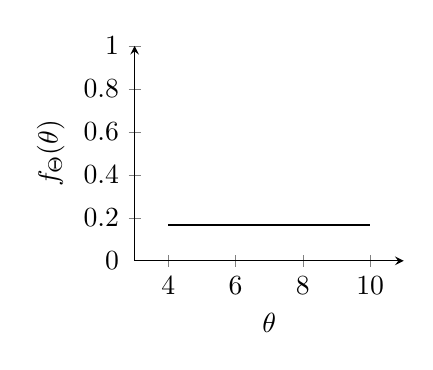
\begin{tikzpicture}
            \begin{axis}[
                axis lines = left,
                xlabel = $\theta$,
                ylabel = {$f_{\Theta}(\theta)$},
                xmin=3, xmax=11,
                ymin=0, ymax=1
            ]
            %define the plot here
            \addplot [
                domain=4:10, 
                samples=2, 
                color=black,
            ]
            {1/6};
            \end{axis}
        \end{tikzpicture}
        \hskip 5pt
        % plot of f(X|theta)
        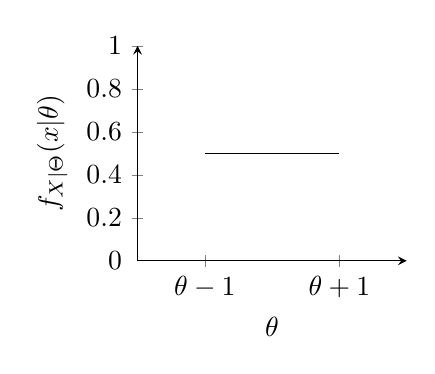
\begin{tikzpicture}
            \begin{axis}[
                axis lines = left,
                xlabel = $\theta$,
                ylabel = {$f_{X|\Theta}(x|\theta)$},
                xmin=0, xmax=4,
                ymin=0, ymax=1,
                xticklabels={$\theta-1$,$\theta+1$},
                xtick={1,3}
            ]
            %define the plot here
            \addplot [
                domain=1:3,
                samples=2, 
                color=black,
            ]
            {1/2};
            \end{axis}
        \end{tikzpicture}
        \hskip 5pt
        % plot of theta vs x
        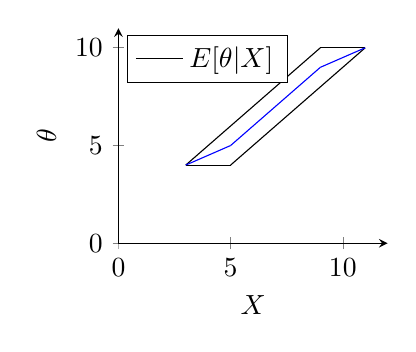
\begin{tikzpicture}
            \begin{axis}[
                axis lines = left,
                xlabel = $X$,
                ylabel = {$\theta$},
                xmin=0, xmax=12,
                ymin=0, ymax=11,
                legend pos=north west,
            ]
            %define the plot here
            \addplot [
                domain=3:5,
                samples=2, 
                color=black,
            ]
            {4};
            \addplot [
                domain=3:9,
                samples=2, 
                color=black,
            ]
            {x+1};
            \addplot [
                domain=9:11,
                samples=2, 
                color=black,
            ]
            {10};
            \addplot [
                domain=5:11,
                samples=2, 
                color=black,
            ]
            {x-1};
            % \addlegendentry{$\theta\;vs\;x$}
            \addplot [
                domain=3:5,
                samples=2, 
                color=blue,
            ]
            {(x/2)+(5/2)};
            \addplot [
                domain=5:9,
                samples=2, 
                color=blue,
            ]
            {x};
            \addplot [
                domain=9:11,
                samples=2, 
                color=blue,
            ]
            {(x/2)+(9/2)};
            \addlegendentry{$E[\theta|X]$}
            \end{axis}
        \end{tikzpicture}

        %%%%%%%%%%%%%%%%%%%%

        %%%%%%%%%%%%%%%%%%%%
        \hypertarget{a_convergence}{\item} \hyperlink{a_convergence}{Question}\newline
        \begin{enumerate}
            \item No, since $X_{i}$ is also uniform in $[-1,1]$
            \item Yes, $E[Y_{i}] = 0$ by symmetry. For $\epsilon > 0$,
            \begin{align*}
                \lim_{i \to \inf}(P\vert Y_{i} - \mu_{i} \vert > \epsilon) &= \lim_{i \to \inf} P(\vert \frac{X_{i}}{i} - 0 \vert > \epsilon)\\
                &= \lim_{i \to \inf} P(\frac{X_{i}}{i} > \epsilon \text{ and } \frac{X_{i}}{i} < -\epsilon)\\
                &= \lim_{i \to \inf} [P(X_{i} > i\epsilon) + P(X_{i} < -i\epsilon)] = 0
            \end{align*}
            \item Yes, $E[Y_{i}] = 0$ by symmetry. For $\epsilon > 0$,
            \begin{align*}
                \lim_{i \to \inf}P(\vert Z_{i} - 0 \vert > \epsilon) &= \lim_{i \to \inf}P((X_{i})^{i} > \epsilon \text{ or } (X_{i})^{i} < -\epsilon)\\
                &= \lim_{i \to \inf} [\frac{1}{2}(1 - \epsilon^{1/i}) + \frac{1}{2}(1 - \epsilon^{1/i})]\\
                &= \lim_{i \to \inf}(1 - \epsilon^{1/i}) = 0
            \end{align*}
        \end{enumerate}
    \end{enumerate}

\end{document}